\documentclass[10pt]{beamer}

\usetheme{metropolis}
\usepackage{appendixnumberbeamer}

\usepackage{booktabs}
\usepackage[scale=2]{ccicons}

\usepackage{pgfplots}
\usepgfplotslibrary{dateplot}

\usepackage{natbib}
\bibpunct[: ]{(}{)}{,}{a}{}{,}
	\newcommand{\BIBand}{\&}
	\setlength{\bibsep}{0pt}
	\setlength{\bibhang}{0.25in}
	\bibliographystyle{sp}
%\bibliographystyle{acm}
%\setlength{\bibhang}{1.8em}

   \newcommand{\posscitet}[1]{\citeauthor{#1}'s (\citeyear{#1})}
    \newcommand{\possciteauthor}[1]{\citeauthor{#1}'s}
    \newcommand{\pgposscitet}[2]{\citeauthor{#1}'s (\citeyear{#1}:~#2)}
    \newcommand{\secposscitet}[2]{\citeauthor{#1}'s (\citeyear{#1}:~$\S$#2)}
    \newcommand{\pgcitealt}[2]{\citealt{#1}:~#2}
    \newcommand{\seccitealt}[2]{\citealt{#1}:~$\S$#2}
    \newcommand{\pgcitep}[2]{(\citealt{#1}:~#2)}
    \newcommand{\seccitep}[2]{(\citealt{#1}:~$\S$#2)}
    \newcommand{\pgcitet}[2]{\citeauthor{#1} (\citeyear{#1}:~#2)}
    \newcommand{\seccitet}[2]{\citeauthor{#1} (\citeyear{#1}:~$\S$#2)}

\usepackage{xspace}
\usepackage{hyperref}
\newcommand{\themename}{\textbf{\textsc{metropolis}}\xspace}

\title{Pohnpei Sohte Ehu}
\subtitle{Quantitative methods for finding emergent heteroglossic patterns in language attitudes}
\date{24 Oct 2017}
\author{Bradley Rentz}
%\institute{Center for modern beamer themes}
% \titlegraphic{\hfill\includegraphics[height=1.5cm]{logo.pdf}}

\begin{document}

\maketitle

\begin{frame}{Kalahngan en\ldots}
\begin{itemize}
\item The Bilinski Foundation
\item My dissertation committee: Andrea, Amy, Christina, Emelihter, and David
\item Carisma, Celine, Cartina, Rofino, Banae, Maynard, Diana, Jade, Carvy, and many others on Pohnpei
\end{itemize}
\end{frame}

\section{Language attitudes background}

\begin{frame}{What are language attitudes?}

\begin{itemize}
\item Language attitudes are the opinions, beliefs, and biases that we have about language use
\item They are the product of social interaction (discourse) \citep{Potter:1987}
\item Can only be observed as an emergent product of discourse
\item Highly contextualized and unstable
\item Are also influenced by all of one's linguistic experiences (education, work, family, friends, geography, politics, etc.)
\end{itemize}
\end{frame}

\begin{frame}{Heteroglossia}
\begin{itemize}
\item An important aspect of the study of language attitudes is the notion of \emph{heteroglossia}
\item Heteroglossia according to \citet{Bakhtin:1981} is the idea that:
\begin{itemize}
\item Every language has internal diversity (whether class, social, ethnic, political, historical, geographic, or otherwise)
\item A community may also have access to other languages as well with their own diversity
\item An individual has multiple voices, whereby they navigate through the complexity of the linguistic resources available to them
\end{itemize}
\item Language attitudes are both a product of heteroglossia and a reinforcer of it
\item Any language attitudes study must take this diversity into account
\end{itemize}
\end{frame}

\section{Quantitative approaches to language attitudes}
\begin{frame}{Past quantitative methods}
\begin{itemize}
\item Typical quantitative research question: what language attitudes do certain groups have and to what extent are they different from other groups
\item Many past language attitudes studies have primarily used regressions and ANOVAs (or ANCOVA, MANOVA, etc.) to analyze group differences
\item These methods require the use of demographic variables to define groups
\end{itemize}
\end{frame}

\begin{frame}{What does regression assume?}
\begin{itemize}
\item The variables used are a meaningful representation of reality
\item There is a single consistent pattern within those groups (aka they approximate a specific normal distribution)
\begin{itemize}
\item There can only be one mean, median, and mode (aka one norm) and deviation from that is noise
\end{itemize}
\item The groups are isolated and are independent of each other
\item Items can only be in one group
\end{itemize}
\end{frame}

\begin{frame}{Problems with demographic variables}
\begin{itemize}
\item Represent social constructs (e.g., age, gender, geographic place, education)
\item Social constructs are messy and have lots of inherent variation
\item Regression assumes an essentialist view of these variables
\item They are often coded with overly simplistic and conservative values (i.e., binary gender)
\item Western colonial constructs are often used instead of potentially more meaningful local categories
\item Require arbitrary cut-offs and groups that may not have any actual behavioral or identity correlates (e.g., age)
\item But can still be useful if done meaningfully
\end{itemize}
\end{frame}

\begin{frame}{Example demographic variable: gender}
\begin{itemize}
\item Do each of the genders exhibit different language attitudes?
\item Imagine all the different women, men, and non-binary people you know
\item How many different opinions, ideologies, and beliefs on a given topic can you think of for each gender?
\item Maybe there are consistent differences at a small level, such as for a single question, but probably not
\item What if there are several different trends that are specific to one gender? 
\end{itemize}
\end{frame}



\begin{frame}{Is regression useful for language attitude studies?}
\begin{itemize}
\item  Yes and no
\item If the demographic variables used correspond to meaningful behaviors where there is a single observable trend for the given groups, then yes
\item If the variables do not represent that, then probably no
\item Regression can miss trends that occur across groups or multiple trends that occur within a single group
\end{itemize}
\end{frame}

\begin{frame}{What can be done instead? MDS and cluster analyses}
\begin{itemize}
\item There are other quantitative analyses that do not have these assumptions
\item Multidimensional scaling (MDS) $+$ cluster analysis allow for patterns to emerge from the data without a priori categories
\item Allows for locally constructed patterns to become visible
\item Shows variation that would have been missed otherwise
\end{itemize}
\end{frame}

\begin{frame}{How does it work?}
\begin{itemize}
\item 3 step process:
\item 1.) Select the applicable response variables and create a dissimilarity matrix
\begin{itemize}
\item This matrix indicate how dissimilar each respondent  is to every other respondent (from 0--1) based on how they responded to those items
\end{itemize}
\item 2.) Apply the MDS algorithm to the dissimilarity matrix
\begin{itemize}
\item This takes the dissimilarity matrix and maps out all the respondents onto a two-dimensional plane
\end{itemize}
\item 3.) Apply a clustering algorithm like Partitioning Around Mediods (PAM)
\begin{itemize}
\item This groups the data into a pre-specified number (k) of clusters
\item k is determined based on the data by looking at the in-cluster variation vs.~between-cluster variation and picking the number of clusters that maximizes the difference \citep{Rousseeuw:1987}
\end{itemize}
\end{itemize}
\end{frame}

\section{Pohnpei case study}

\begin{frame}{Pohnpei sohte ehu}
\begin{itemize}
\item Pohnpei sohte ehu (Pohnpei is not one) is a common metaphor on the island
\item Contrary to most views of `Micronesia', Pohnpei is a place of high linguistic diversity and multilingualism
\item This study (my dissertation) has 301 respondents (1.3\% of the adult population)
\item Respondents reported speaking over 30 languages 
\item Median number of languages spoken per respondent is 3
\end{itemize}
\end{frame}

\begin{frame}{Map of respondents}
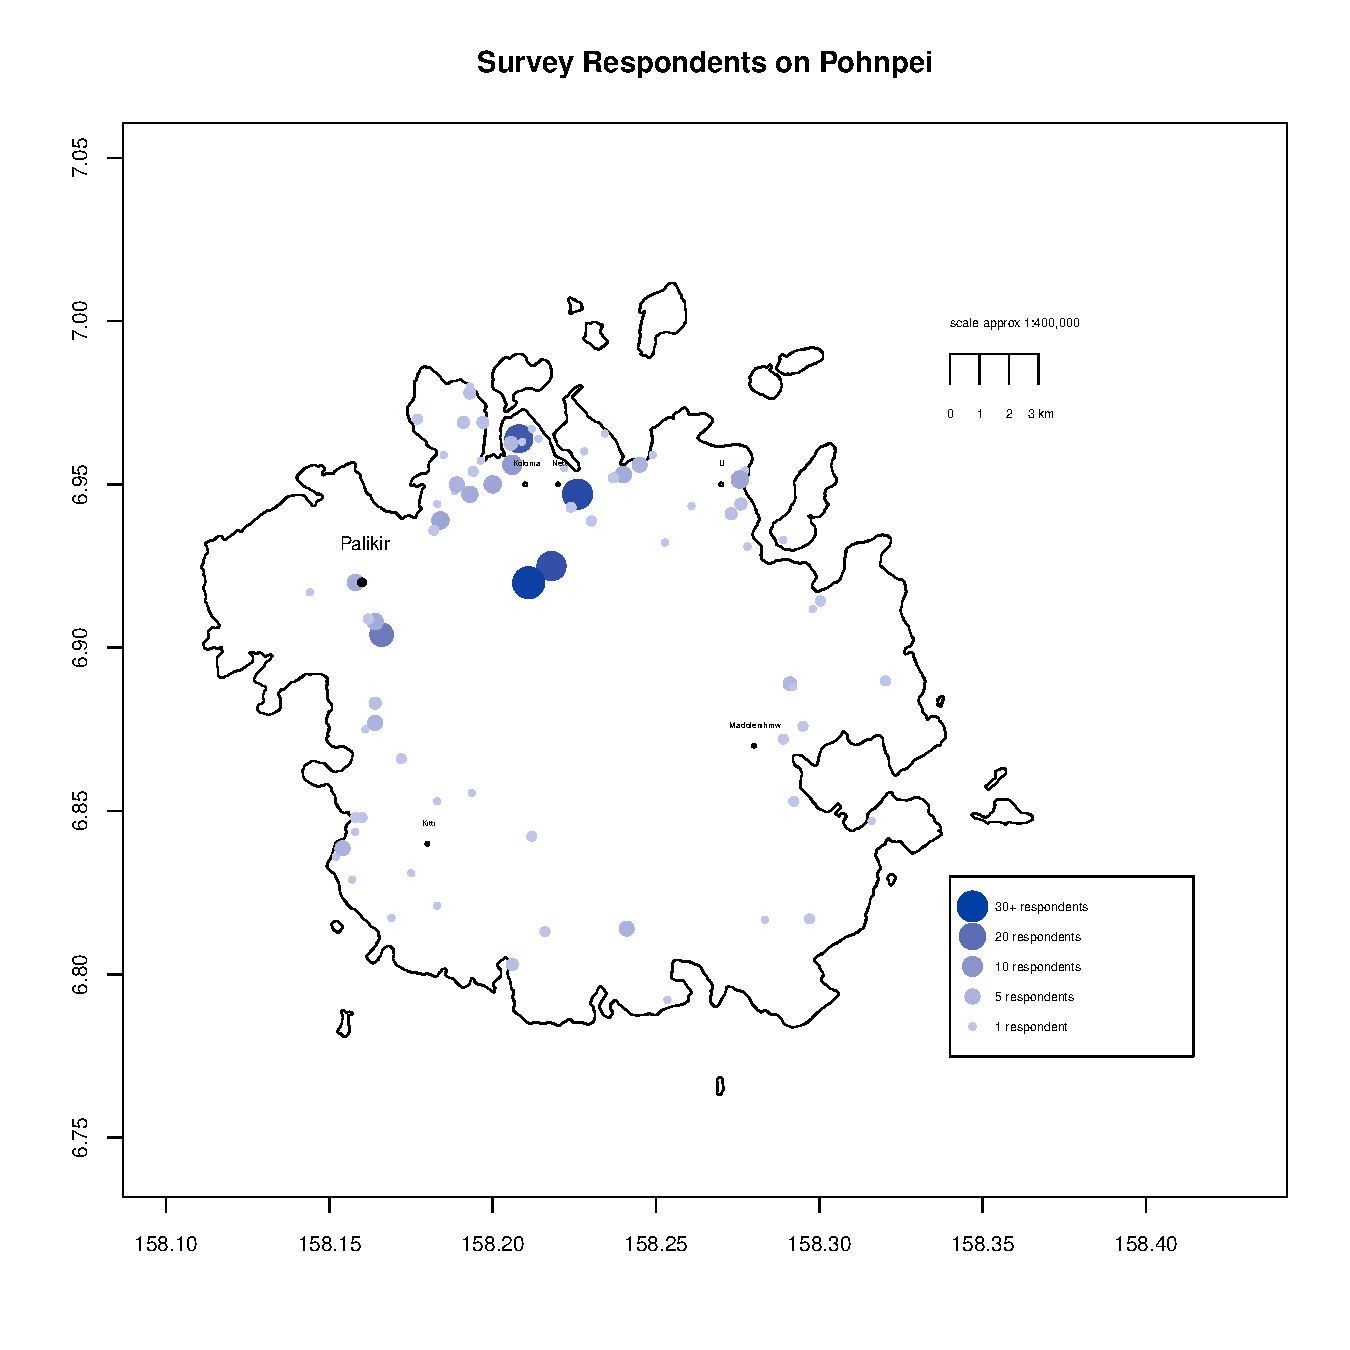
\includegraphics[width=0.75\textwidth]{figures/participantMap.pdf}
\end{frame}


\begin{frame}{First languages of respondents}
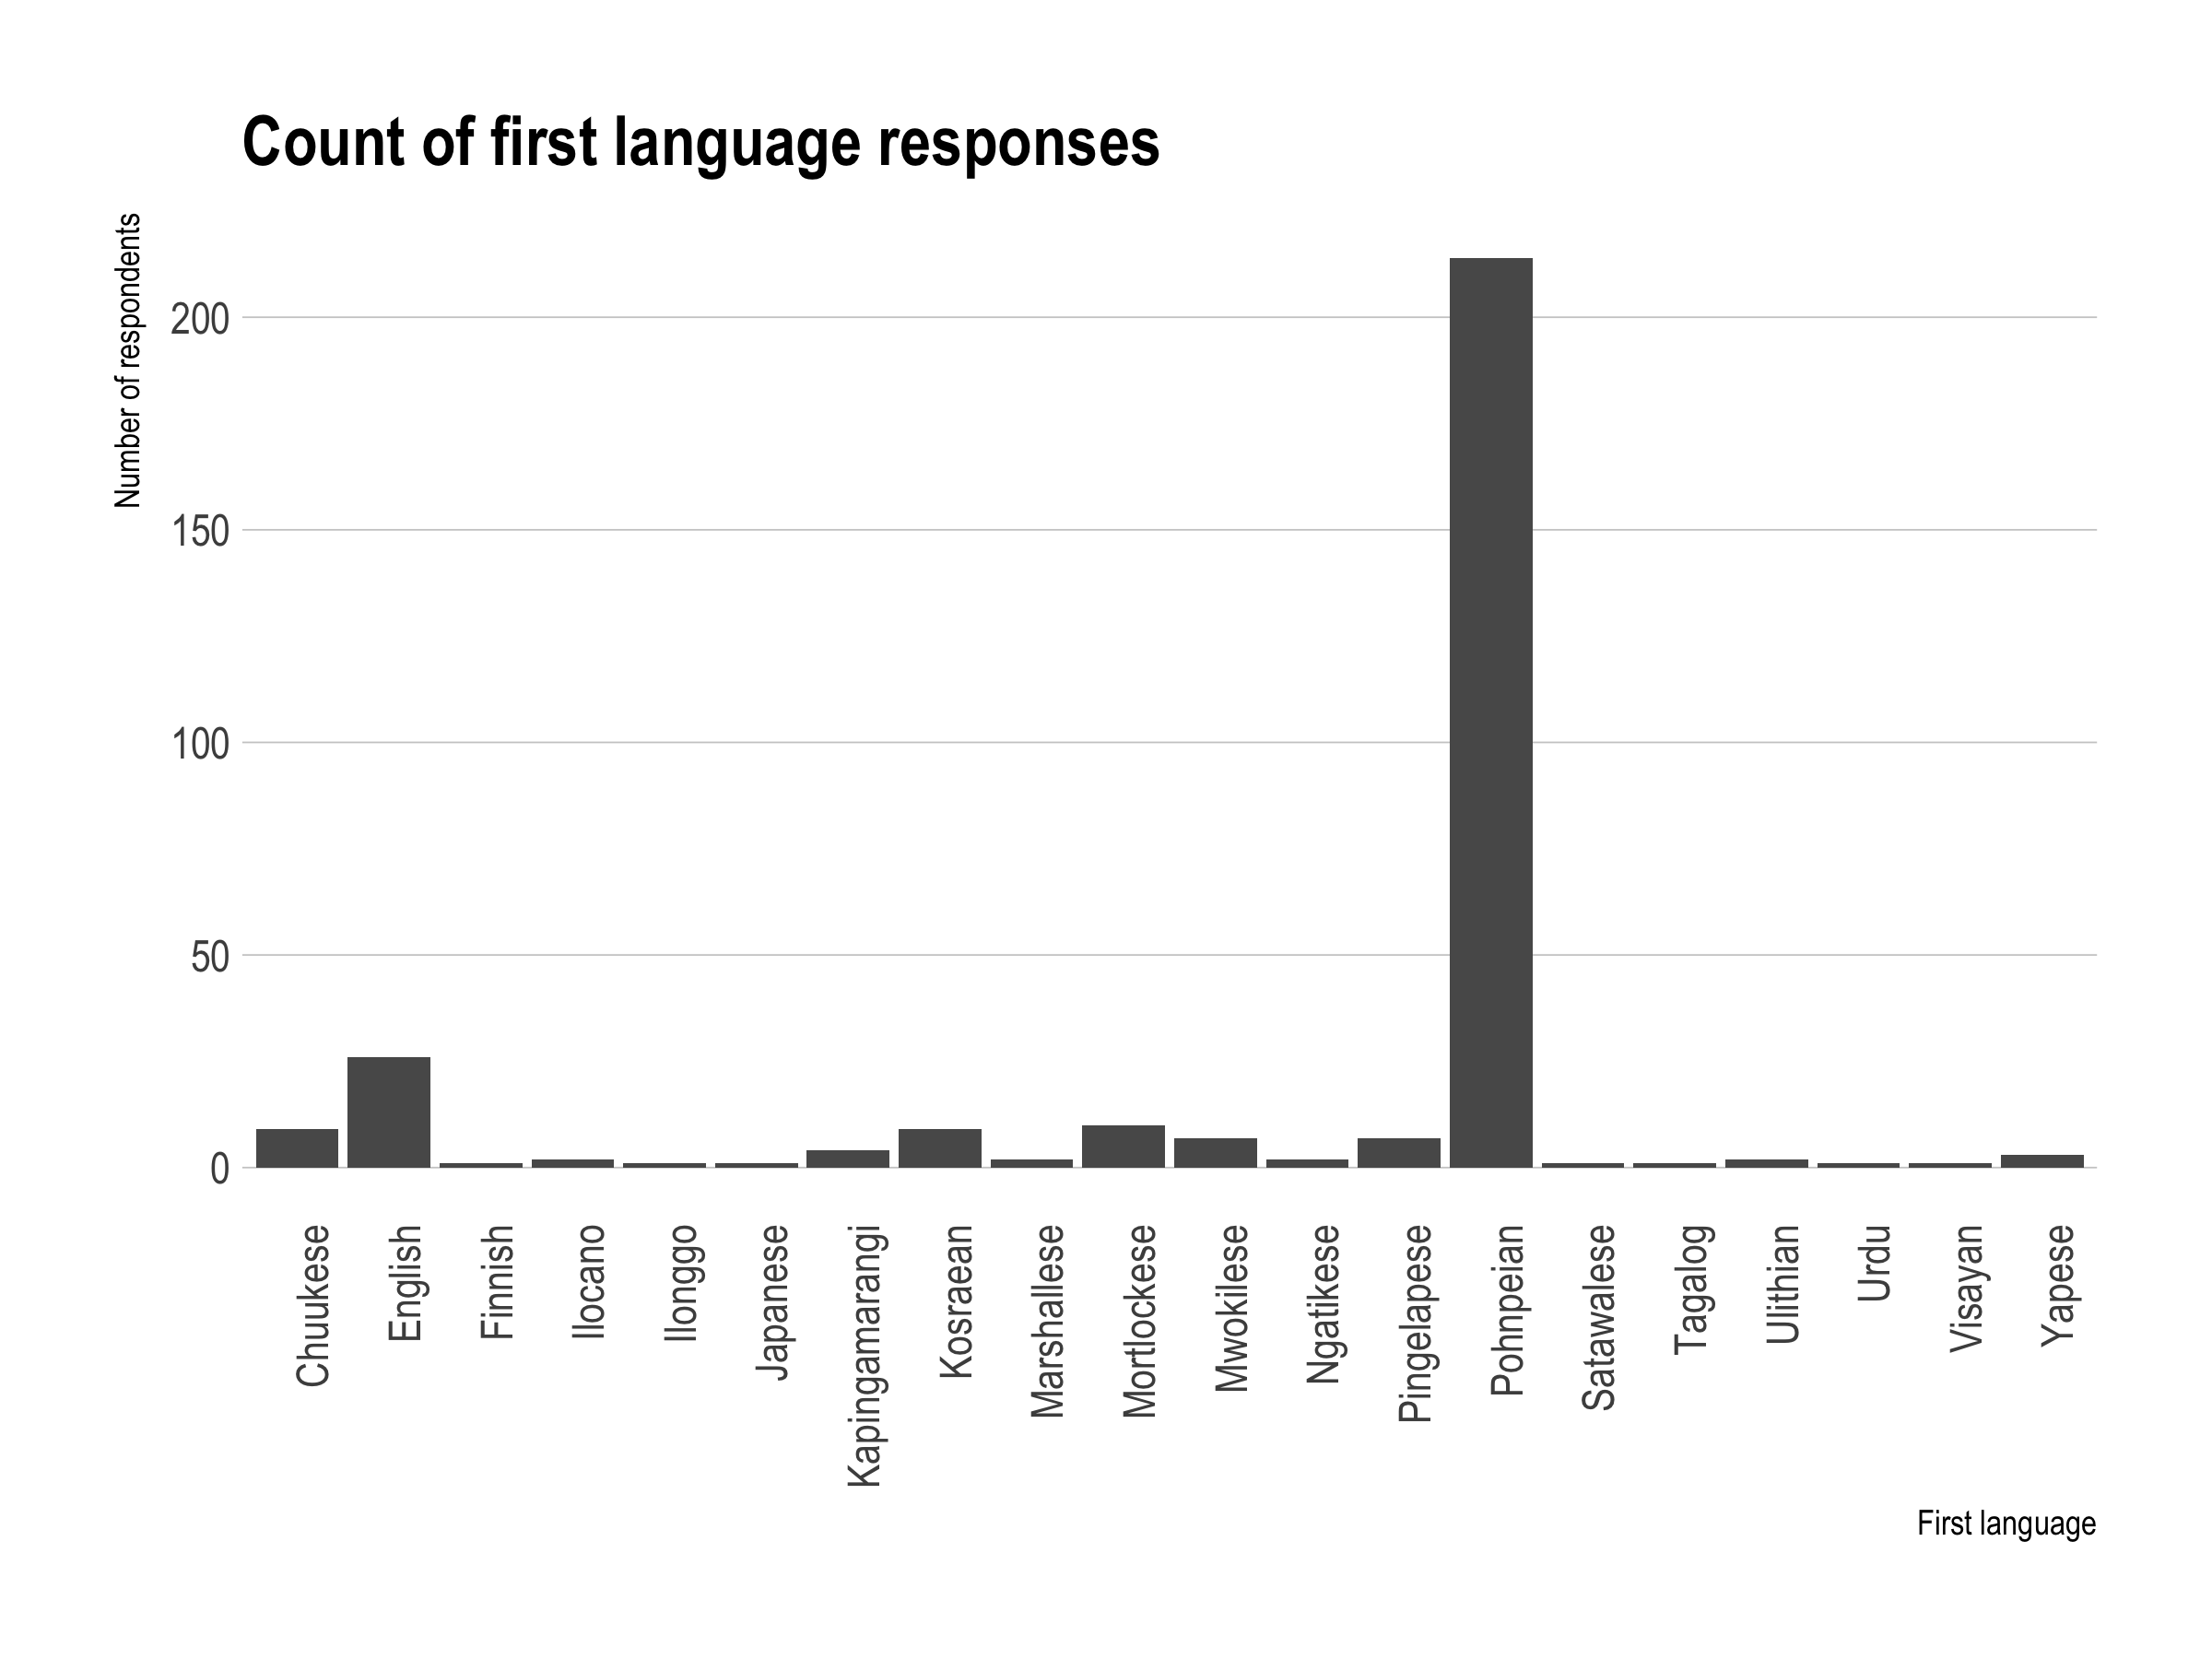
\includegraphics[width=0.9\textwidth]{figures/L1.png}
\end{frame}

\begin{frame}{L2s spoken well by respondents}
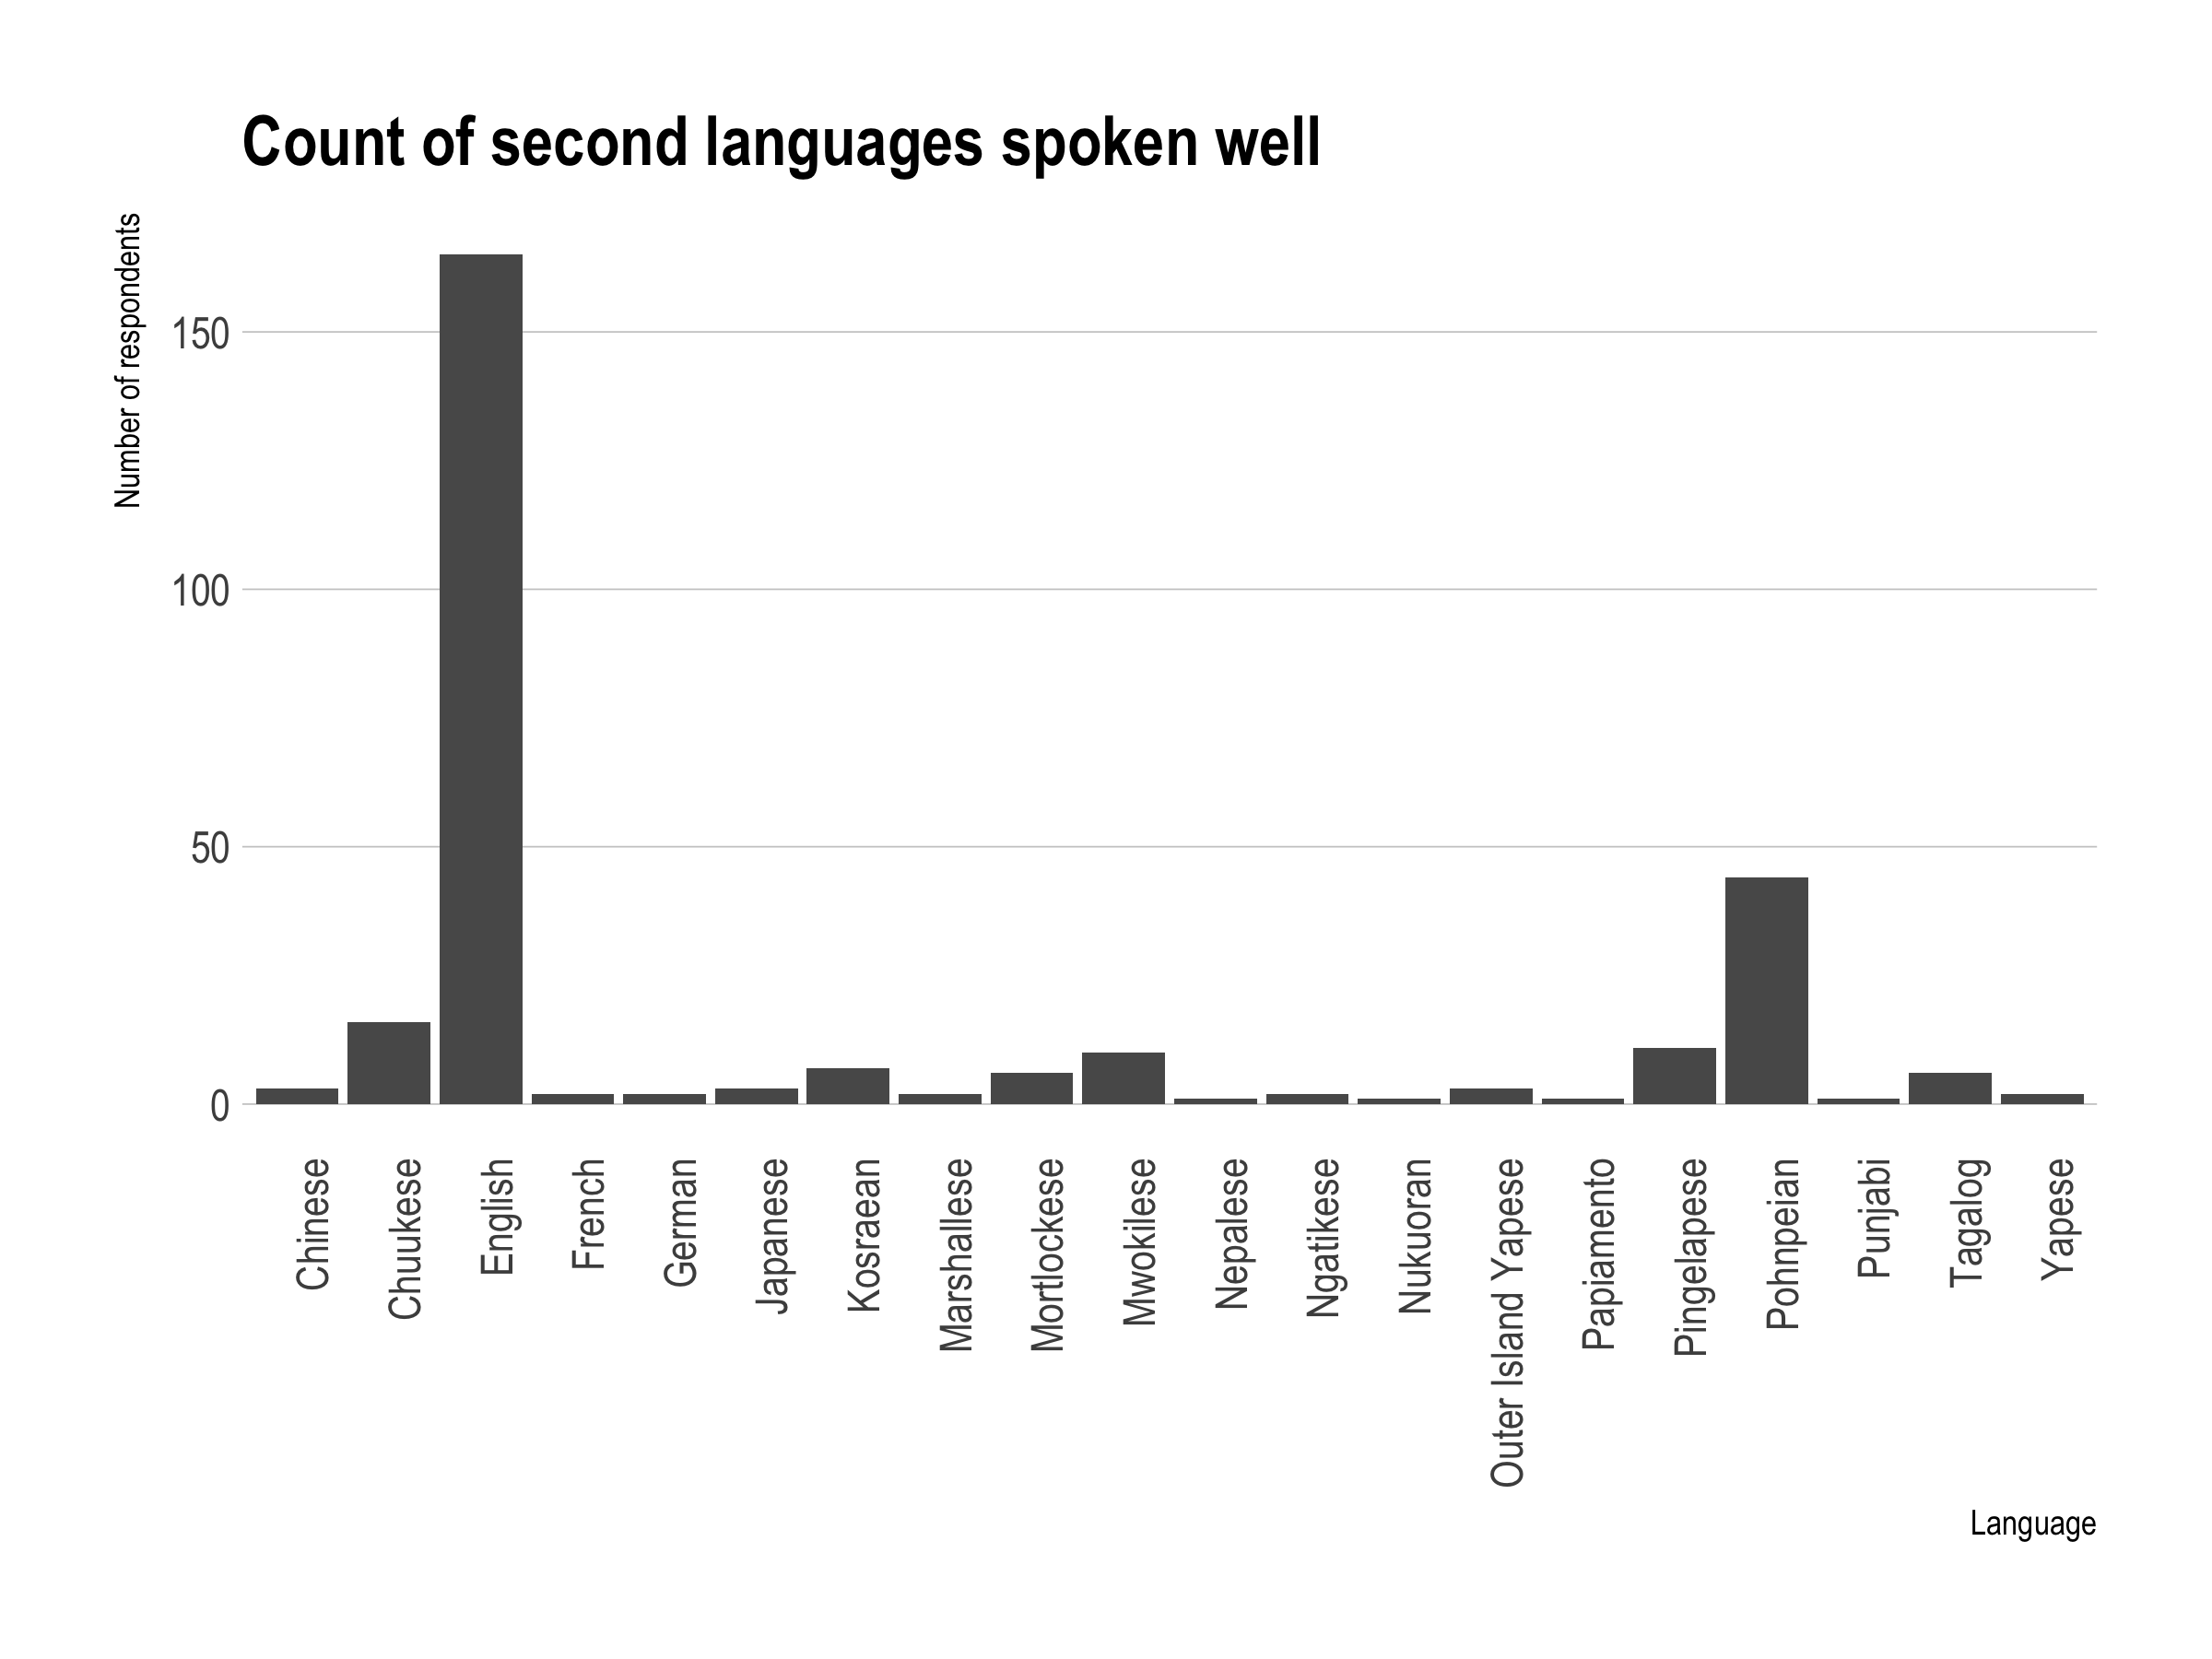
\includegraphics[width=0.9\textwidth]{figures/L2well.png}
\end{frame}

\begin{frame}{L2s spoken a little by respondents}
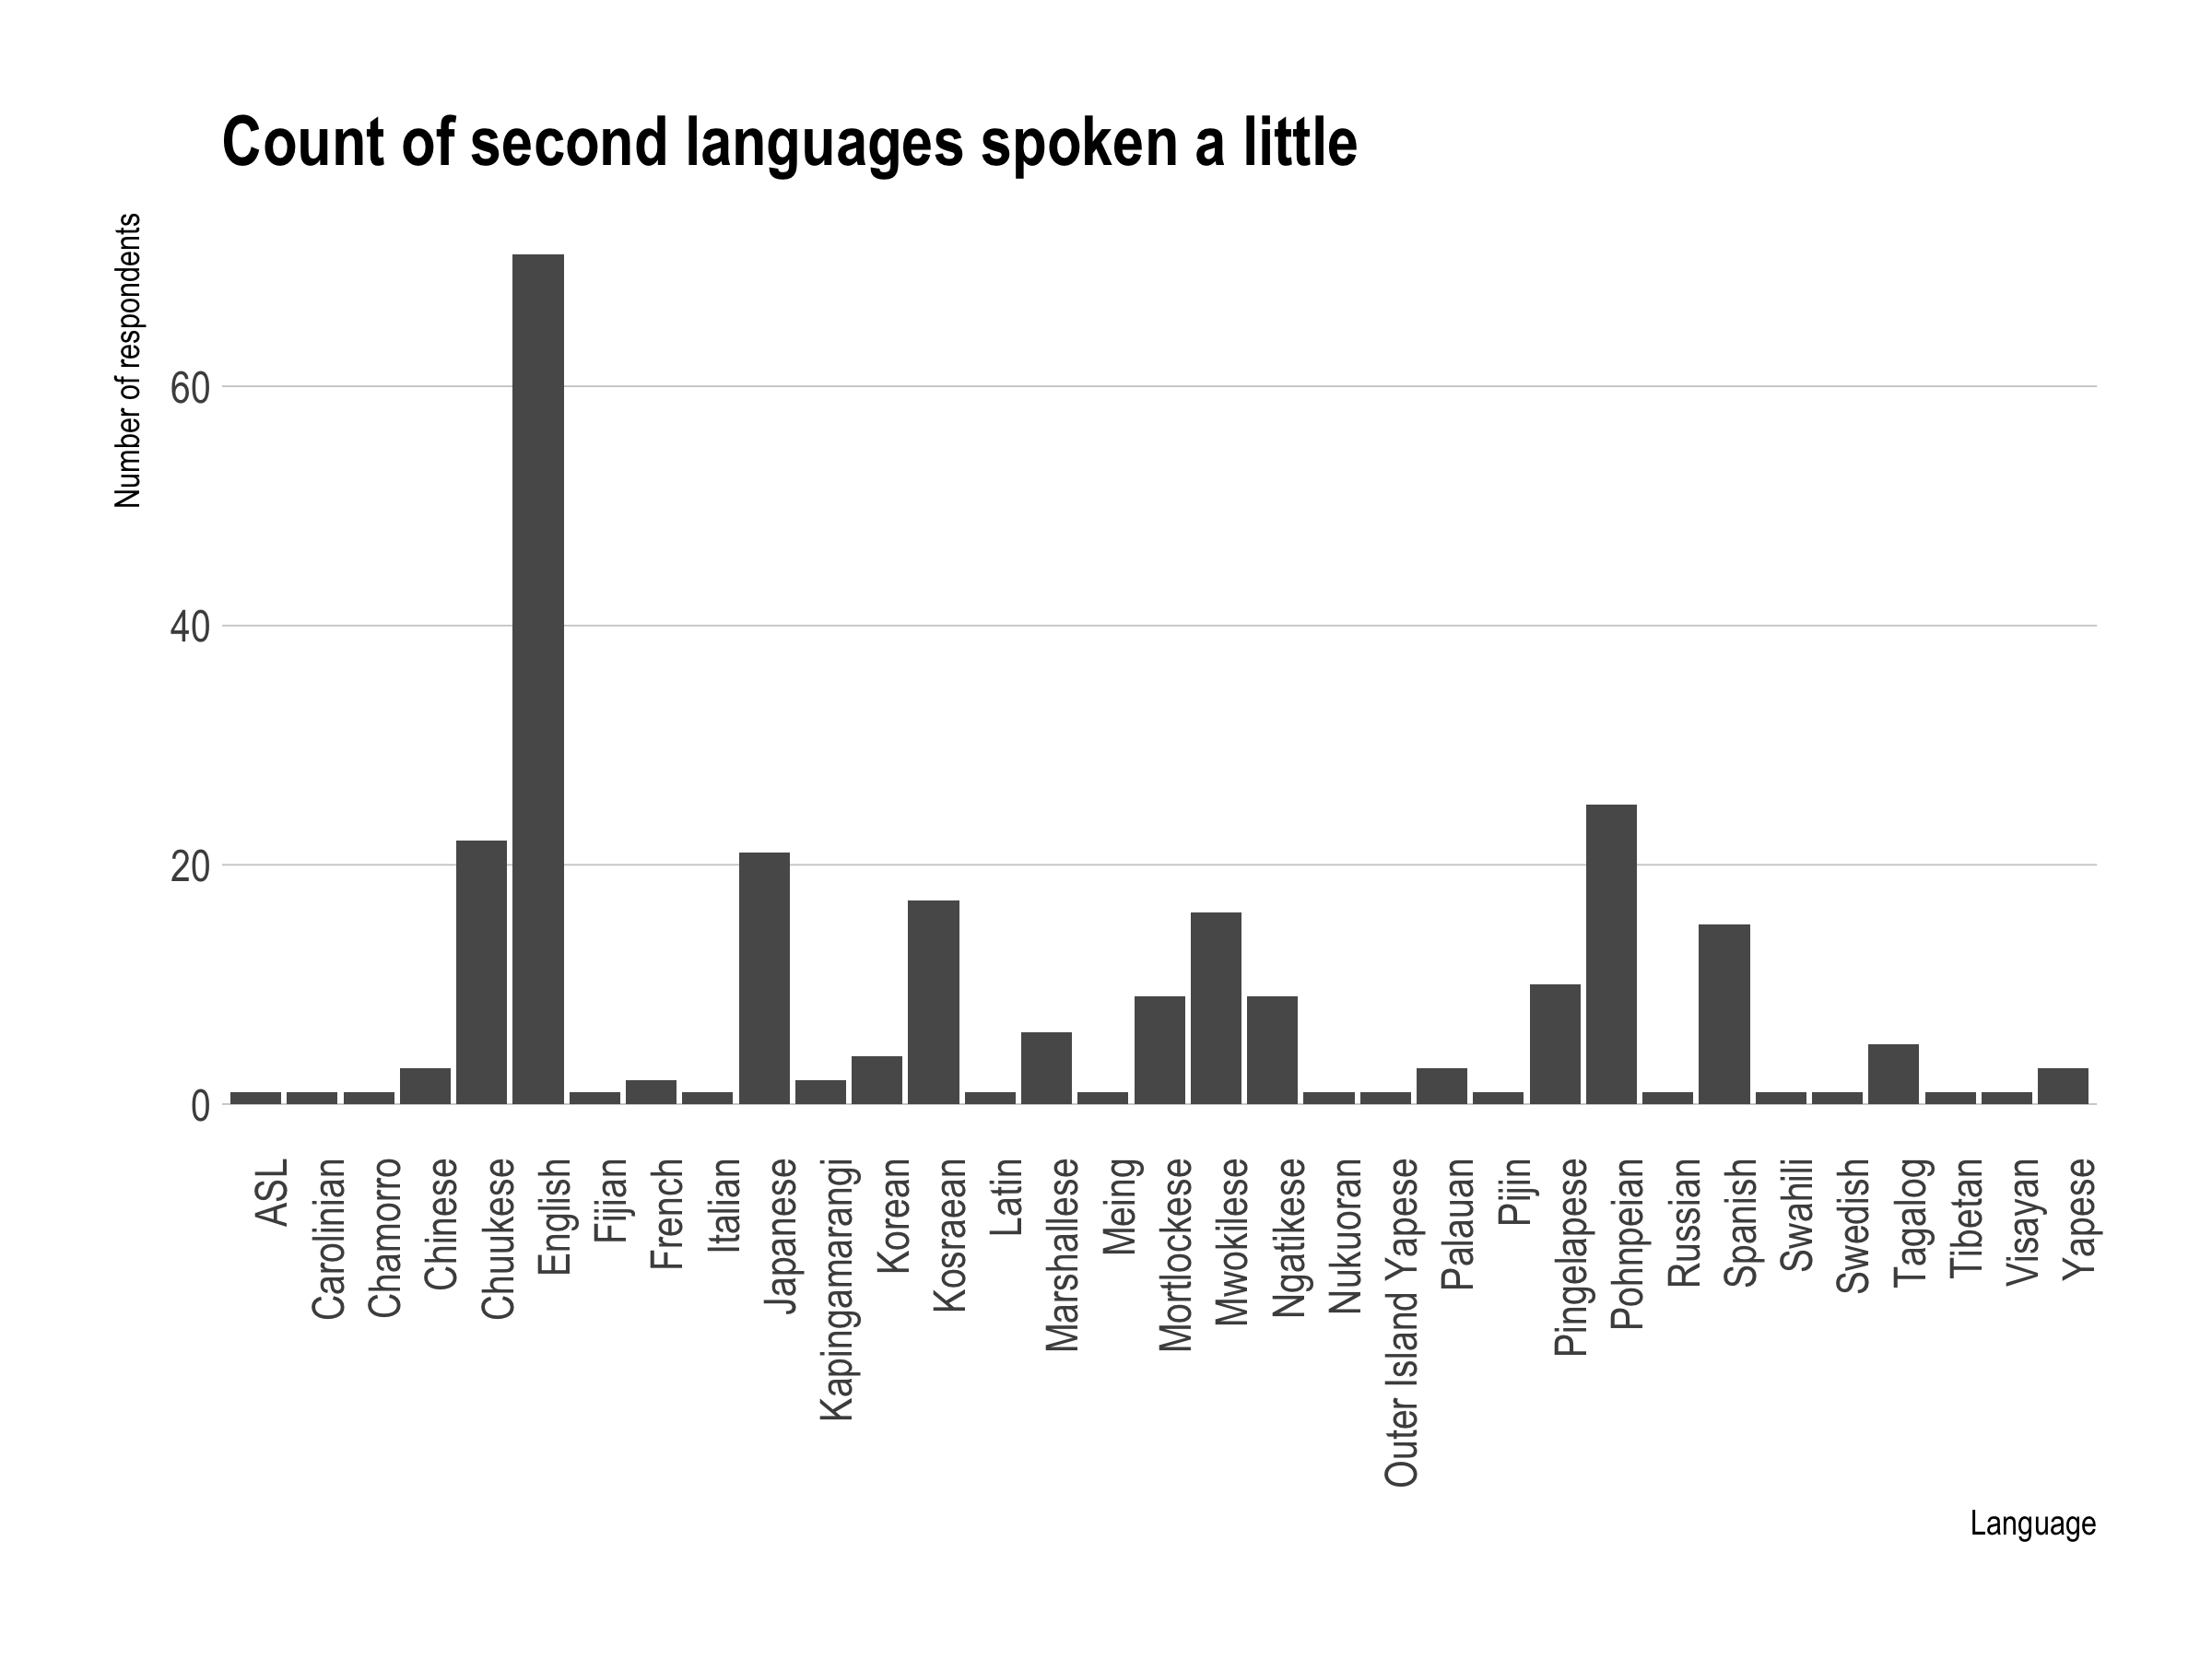
\includegraphics[width=0.9\textwidth]{figures/L2little.png}
\end{frame}

\section{Domain-based language attitudes}

\begin{frame}{Domain-based language importance}
\begin{itemize}
\item Respondents were asked to select 1 of 8 languages that is most important  for 25 different domains
\item These questions were analyzed via Bayesian hierarchical regression modeling and MDS $+$ PAM
\end{itemize}
\end{frame}


\begin{frame}{Regression}
\begin{itemize}
\item Dependent variable: The number of times a respondent selected English for any of the 25 domains (0--25)
\item Predictor variables: age, gender, birth location, travel abroad, years on Pohnpei, ability to speak the formal registers of Pohnpeian (Meing), education achievement level, elementary school type (public or private), high school type (public, private, or none)
\item Mixed effects: Current section of island nested in current municipality
\item Includes poststratification survey weights
\item Predictors deviation coded
\end{itemize}
\end{frame}

\begin{frame}{Posterior distributions for age and gender}
\begin{tabular}{lrrrrl}

  \toprule
Parameter & mean & sd & 2.5\% & 97.5\% & Meaning of predictor \\
  \midrule
(Intercept) & 11.8 & 2.2 & 7.1 & 15.8 & Grand mean \\
  age1 & 2.8 & 1.5 & -0.1 & 5.6 & 18--24 years old \\
  age2 & 0.9 & 1.2 & -1.5 & 3.4 & 25--34 years old \\
  age3 & -0.8 & 1.0 & -2.8 & 1.2 &  35--45 years old \\
  age4 & -1.6 & 1.1 & -3.7 & 0.6 &45--54 years old  \\
  age5 & 1.3 & 1.3 & -1.2 & 3.8 & 55--64 years old  \\
  age6 & -0.2 & 1.9 & -3.8 & 3.6 & 65--74 years old\\
  sex1 & 0.2 & 0.4 & -0.5 & 1.0 & women \\
  \bottomrule
  \end{tabular}
  \end{frame}

\begin{frame}{Posterior distributions for age and gender}
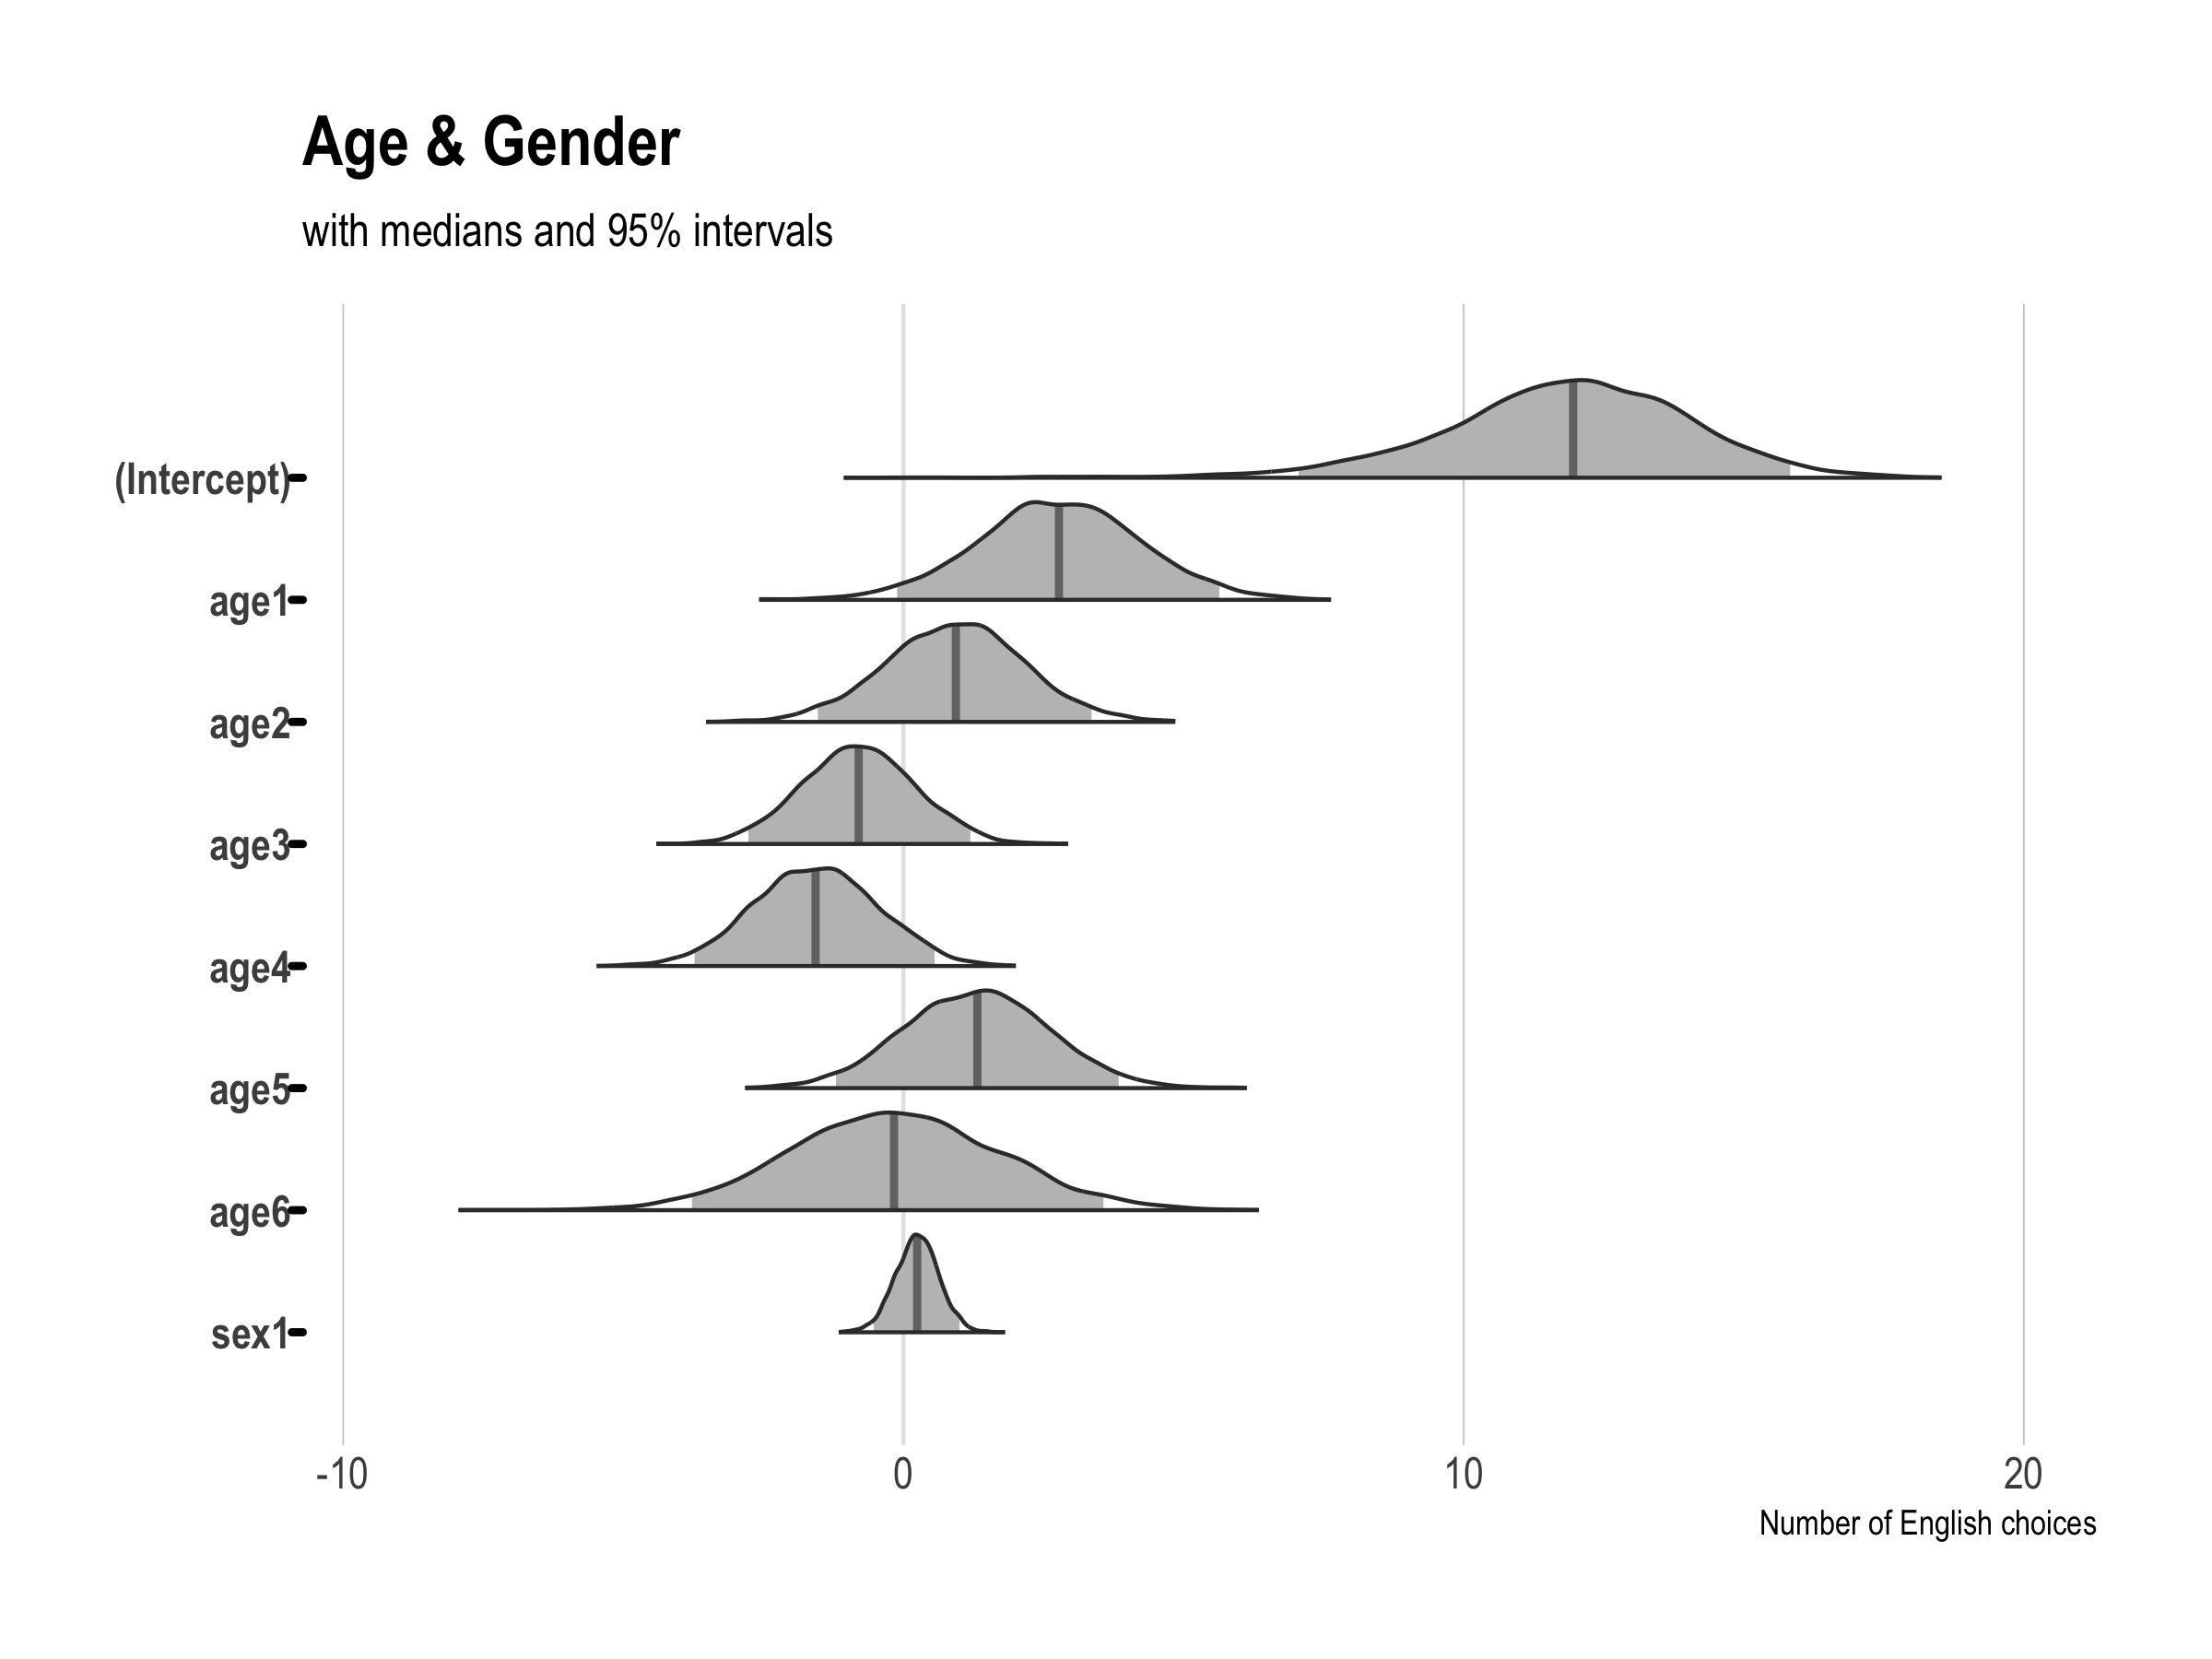
\includegraphics[width=0.9\textwidth]{figures/engAgeGender.png}
\end{frame}



\begin{frame}{Age and Gender}
\begin{itemize}
\item There are some differences by age group but not a linear trend (stops with age5 and age6) and high variation
\item Little to no difference based on gender
\item Are these useful categories? 
\begin{itemize}
\item Do show some differences
\item But these are large groups with lots of inherent variation that is not seen
\item Gender has so much internal variation that it is no different from the grand mean
\end{itemize}
\end{itemize}
\end{frame}

\begin{frame}{RDI plot of English choices by gender}
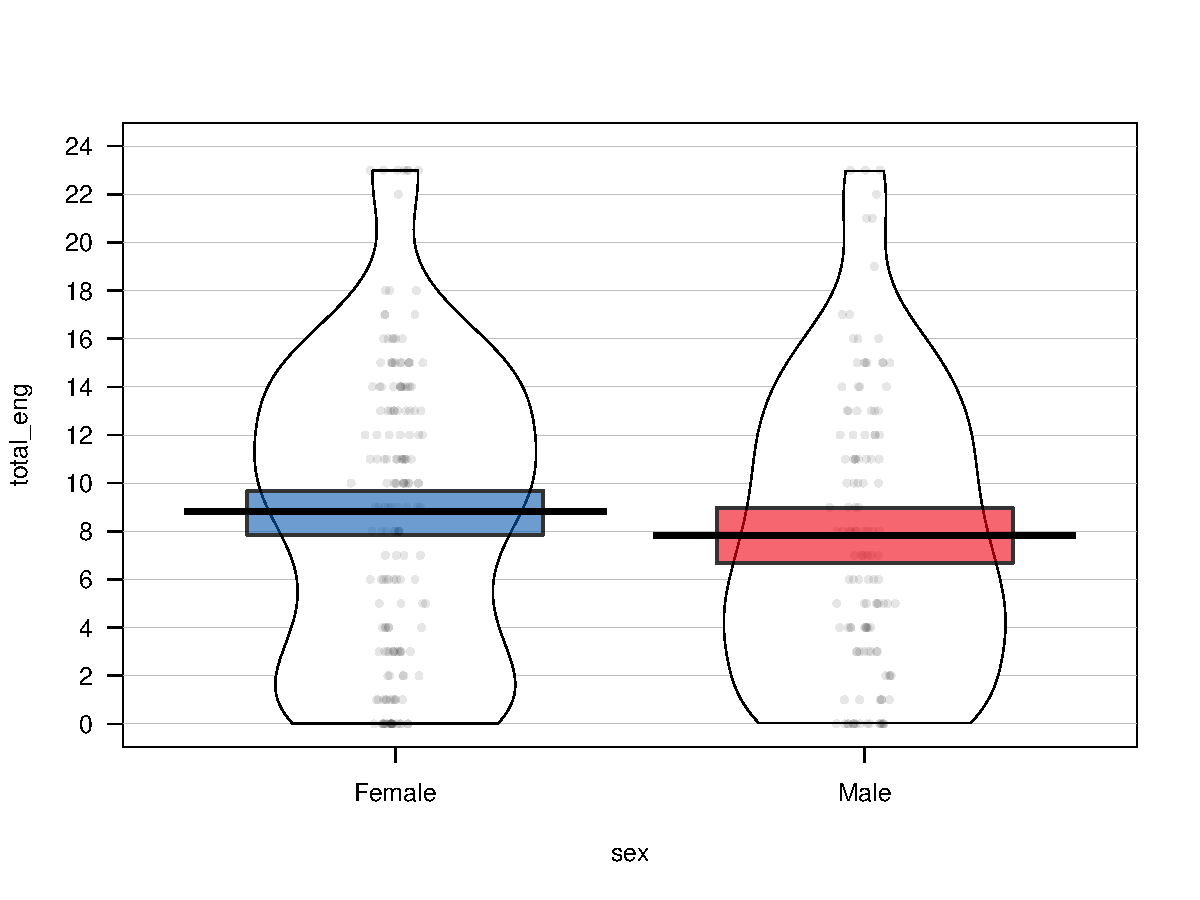
\includegraphics[width=0.9\textwidth]{figures/engHDIgender.pdf}
\end{frame}



\begin{frame}{MDS and PAM}
\begin{itemize}
\item Clustered all of the respondents into two groups based on their responses to the 25 questions
\item Number of groups was determined by the data and not a priori
\item Questions are grouped into 6 super-domains for display purposes: education, occupation, general, media, and social solidarity
\end{itemize}
\end{frame}

\begin{frame}{MDS and PAM}
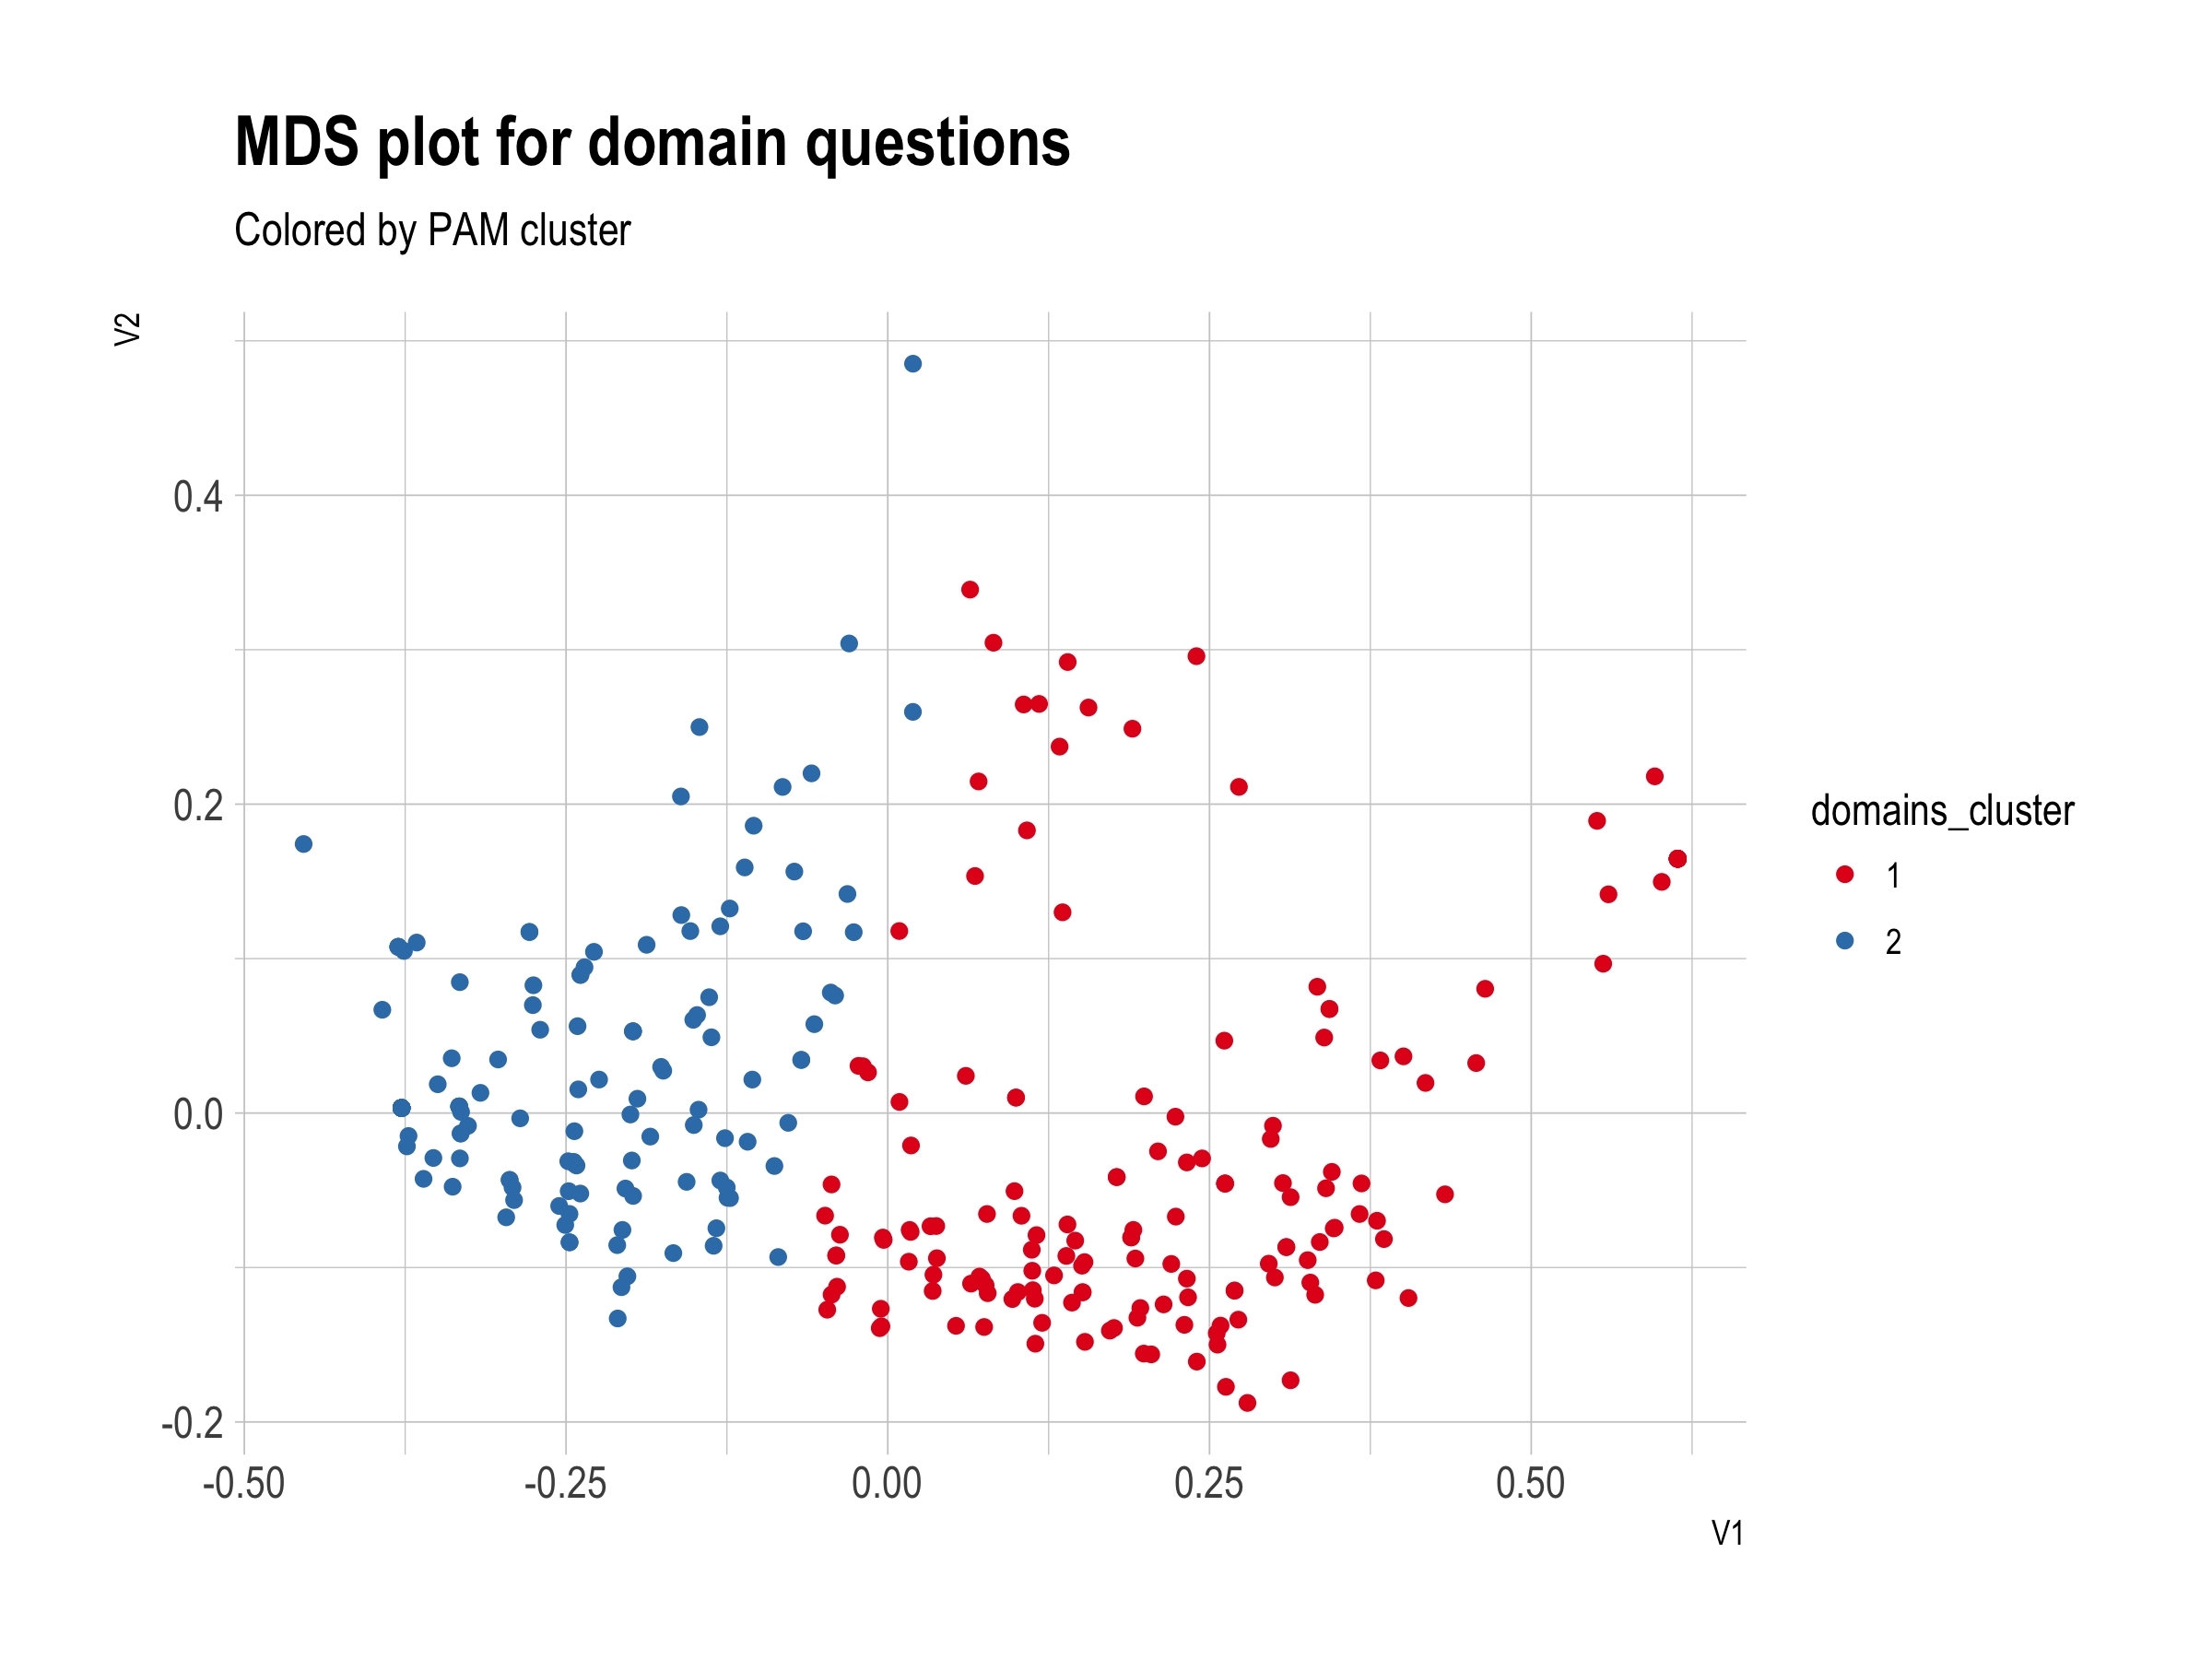
\includegraphics[width=0.9\textwidth]{figures/mdsdomainspam.png}
\end{frame}

\begin{frame}{Education domains (original)}
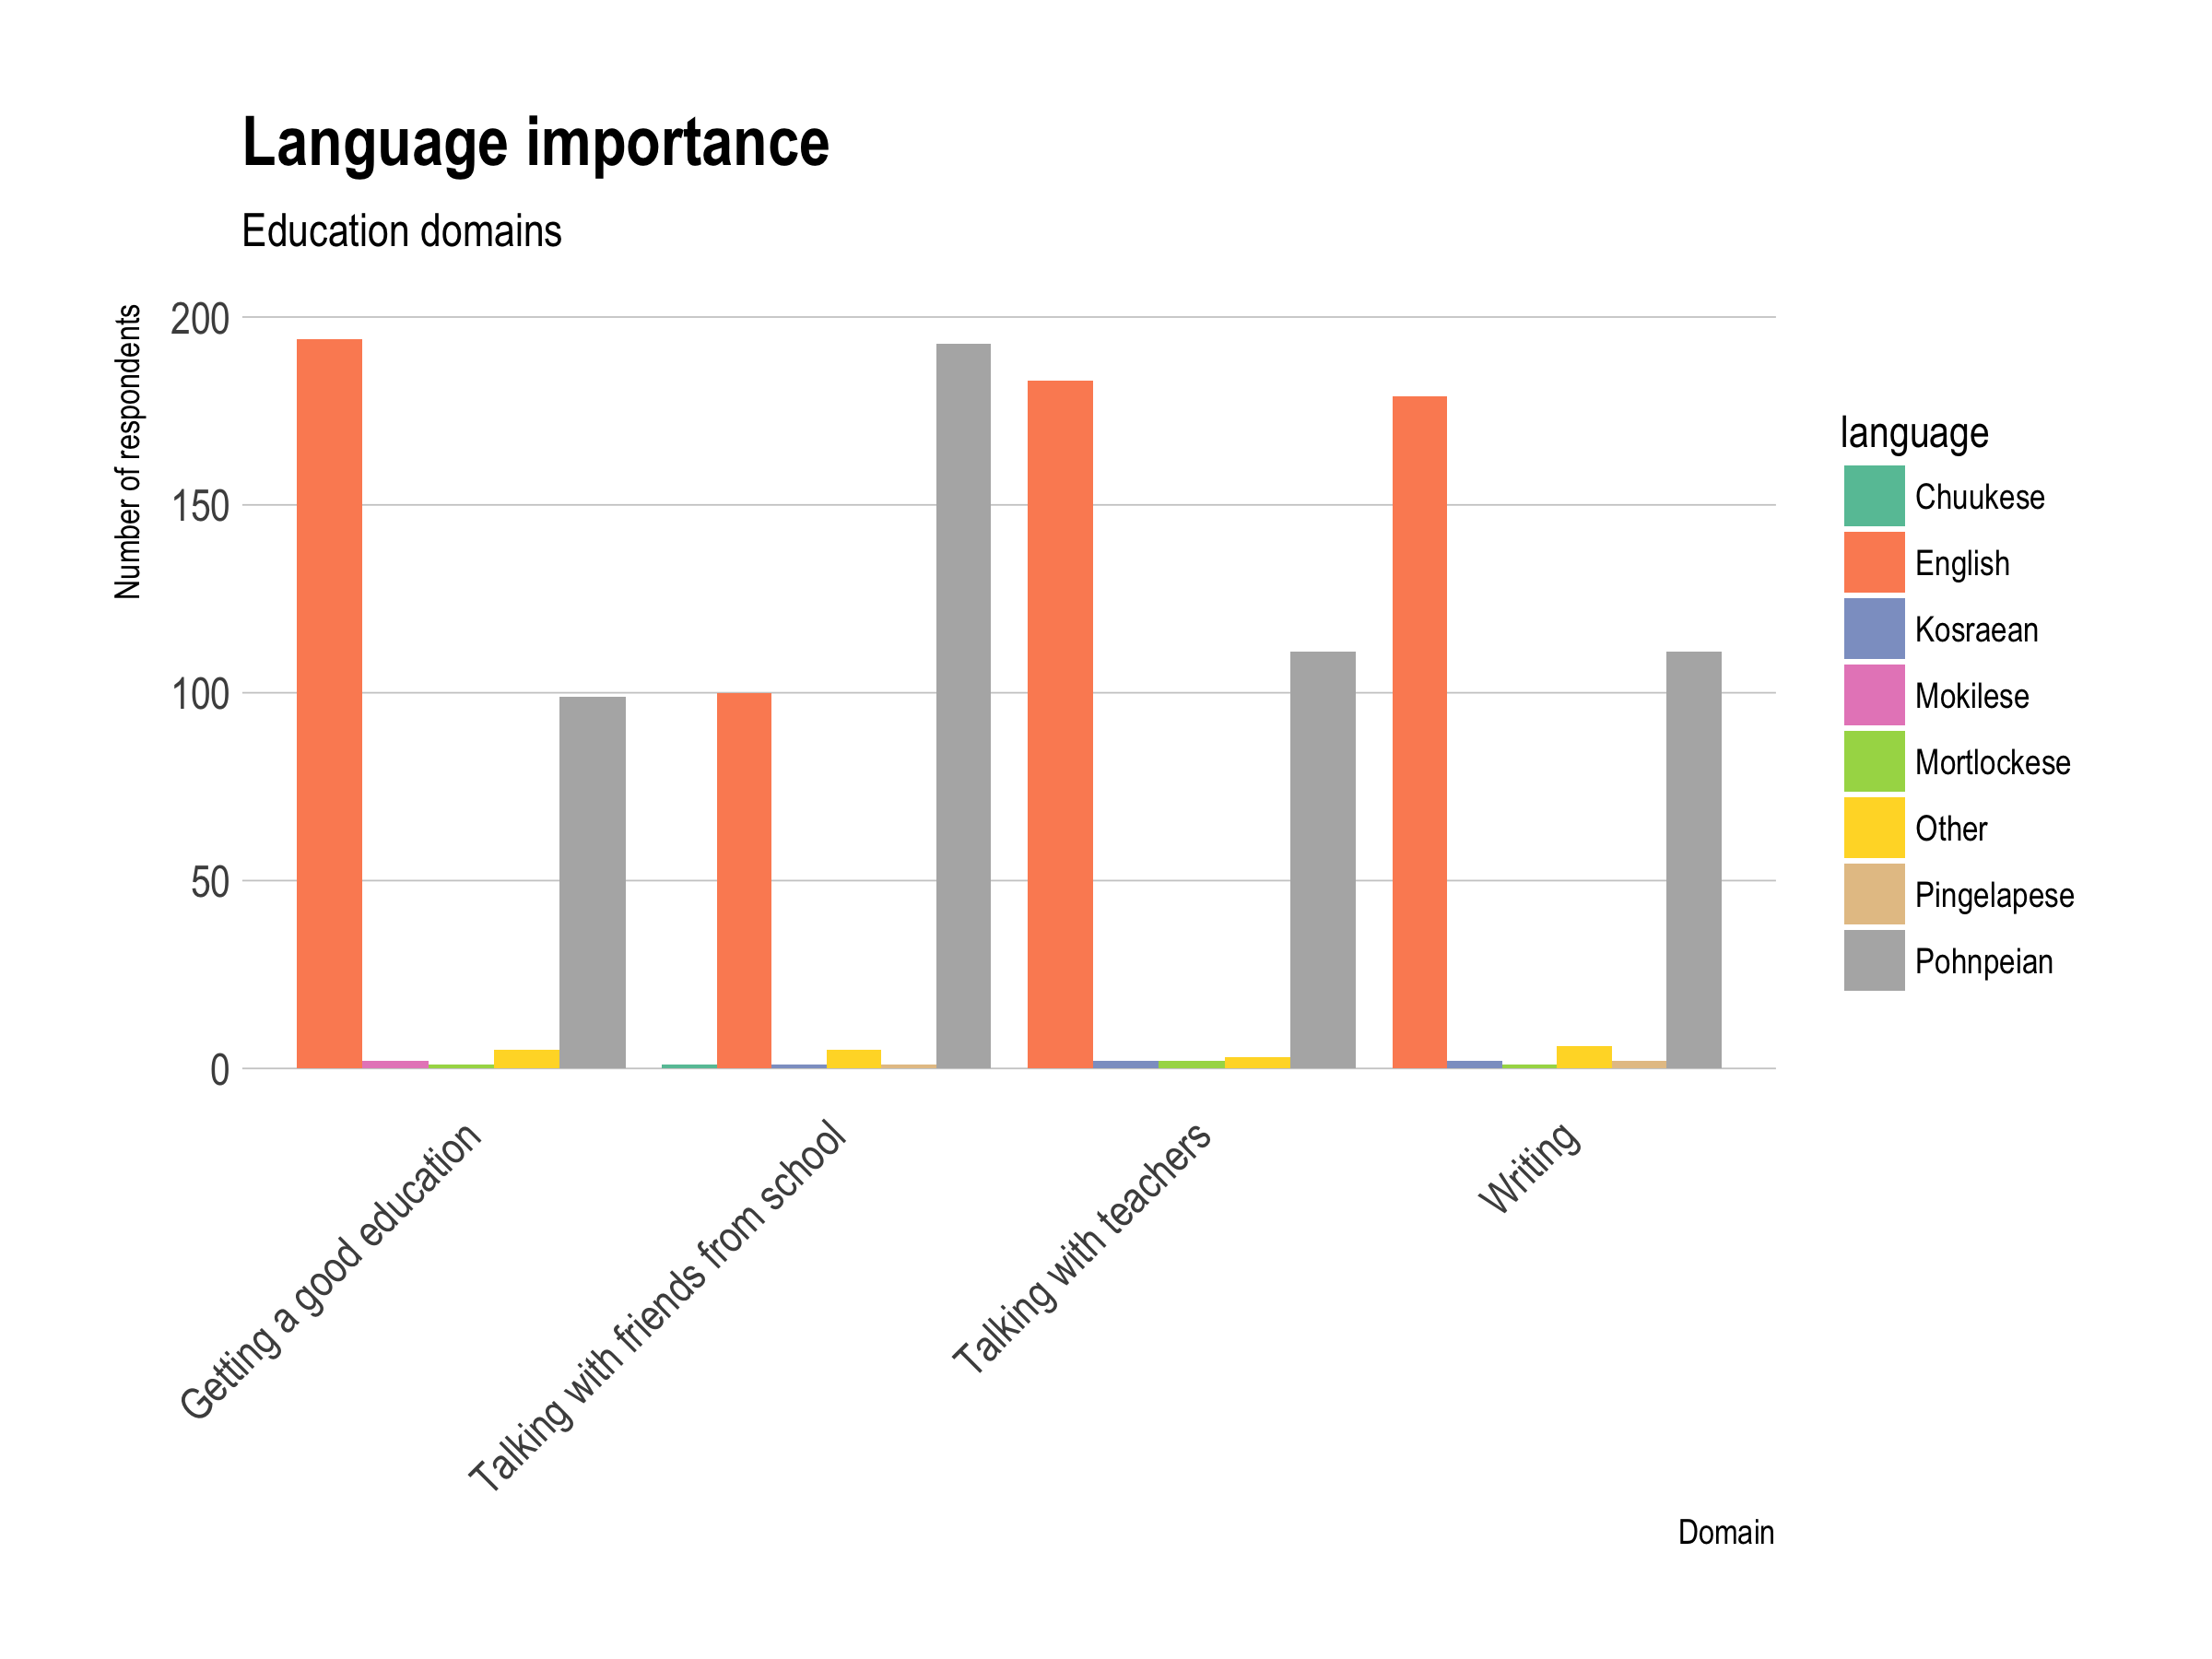
\includegraphics[width=0.9\textwidth]{figures/educationdomains.png}
\end{frame}

\begin{frame}{PAM Education domains}
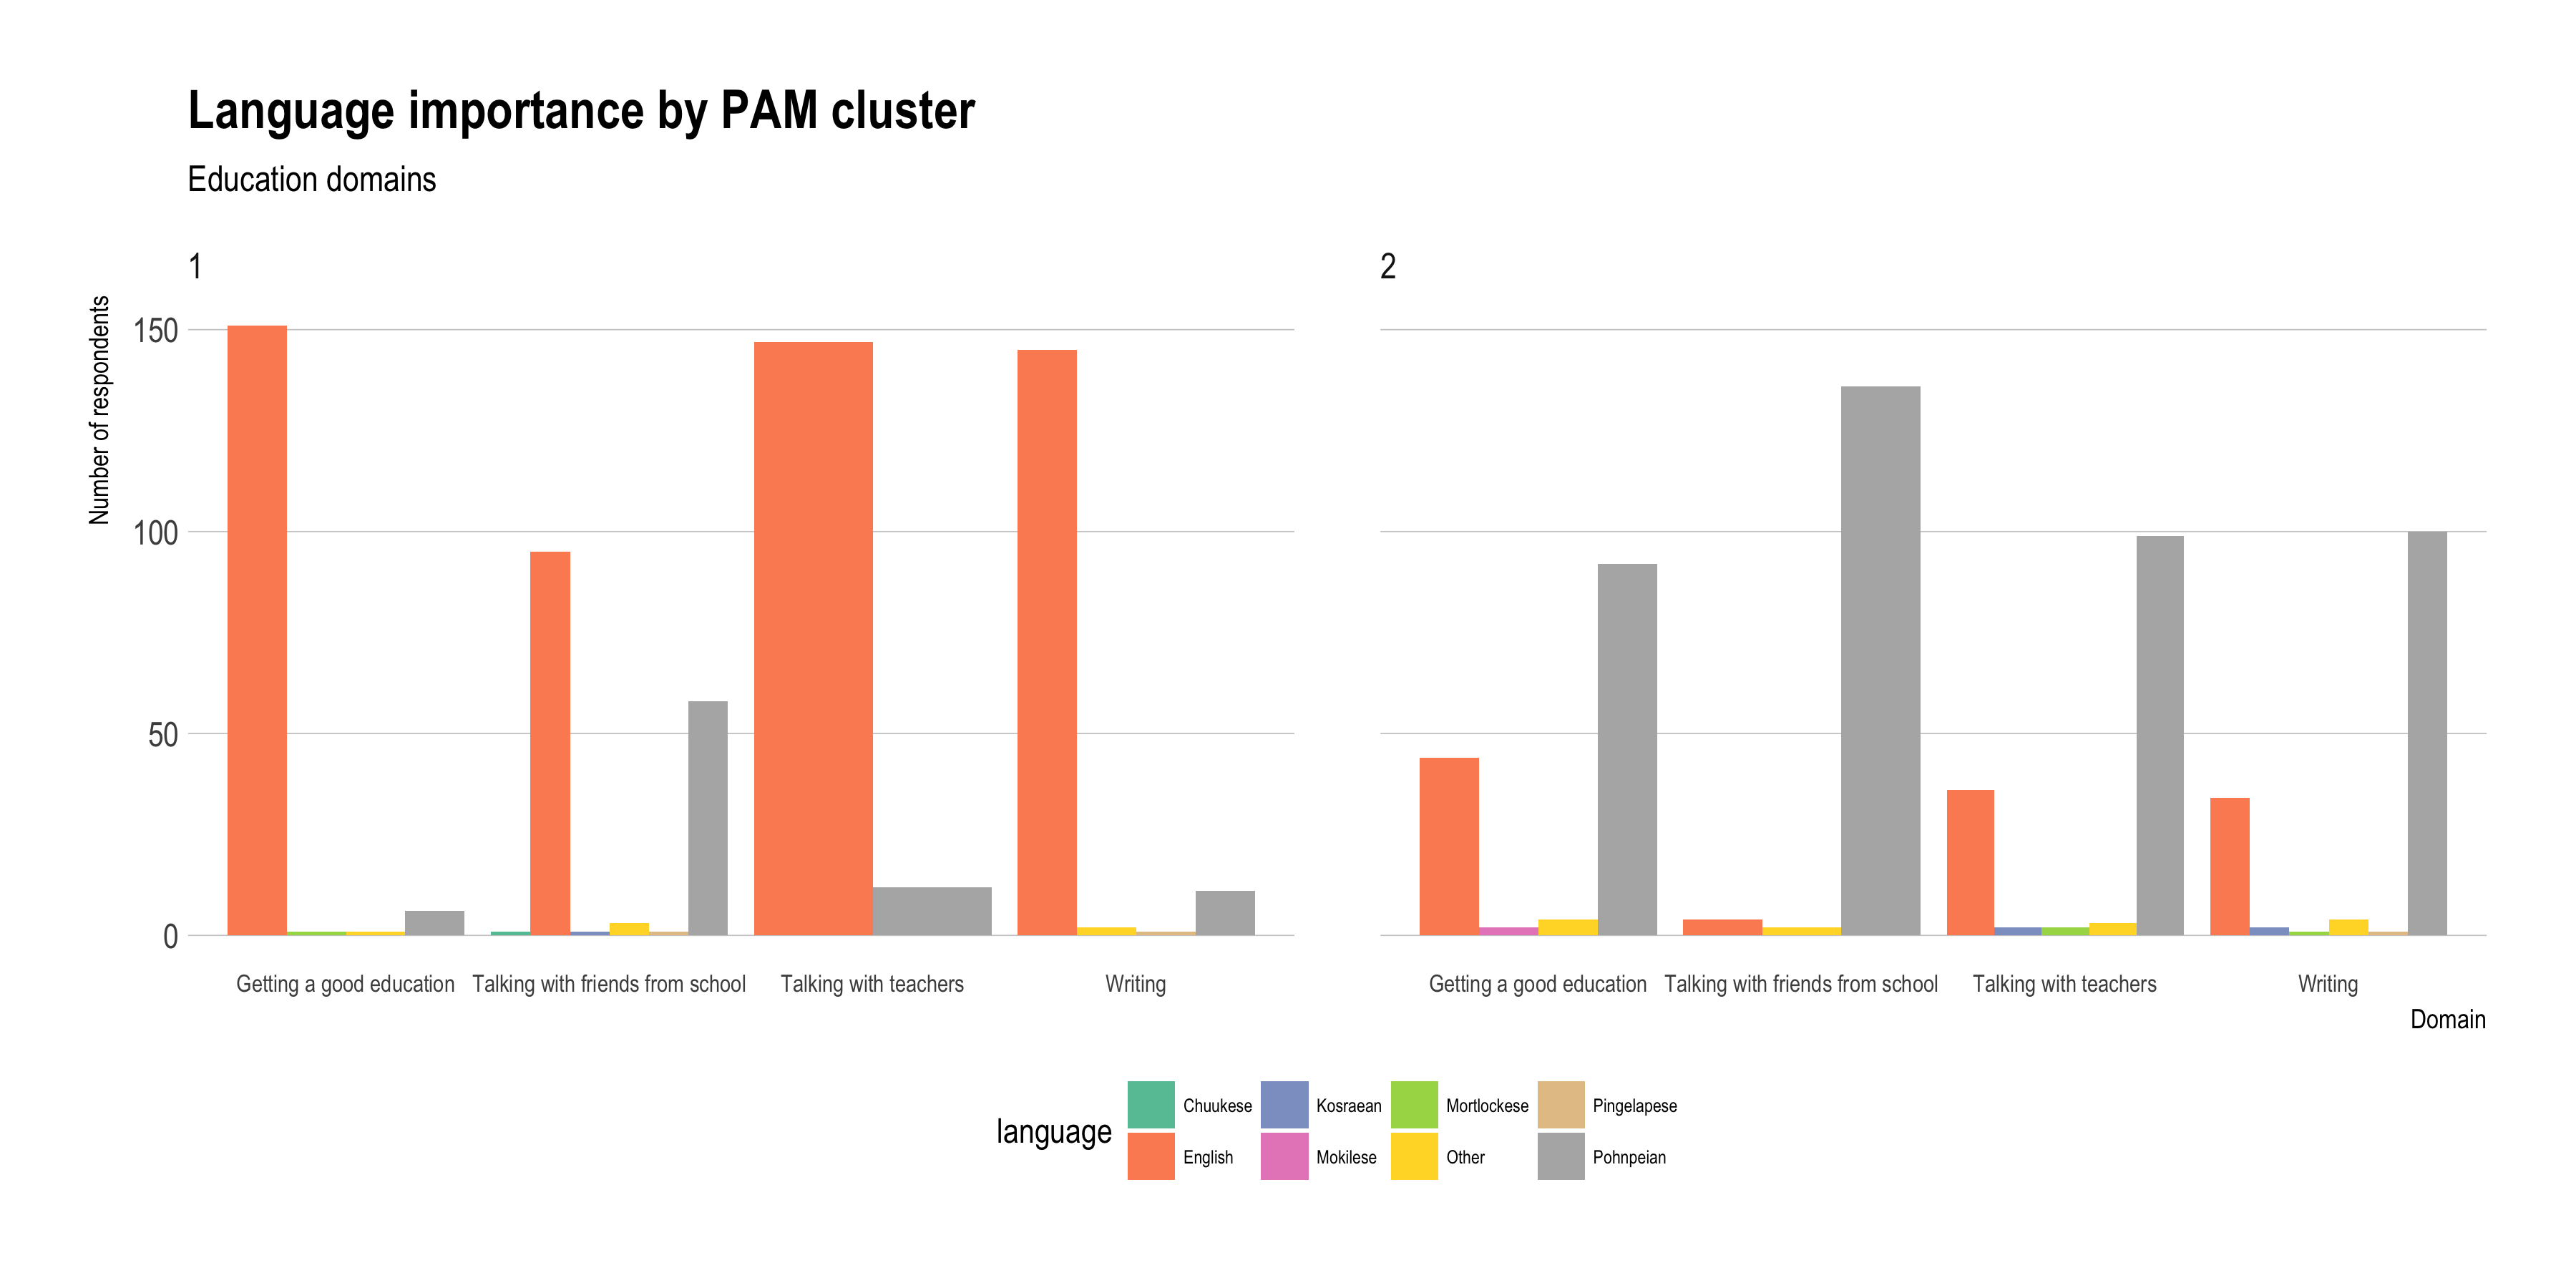
\includegraphics[width=0.95\textwidth]{figures/PAMeducationdomains.png}
\end{frame}

\begin{frame}{Occupation domains (original)}
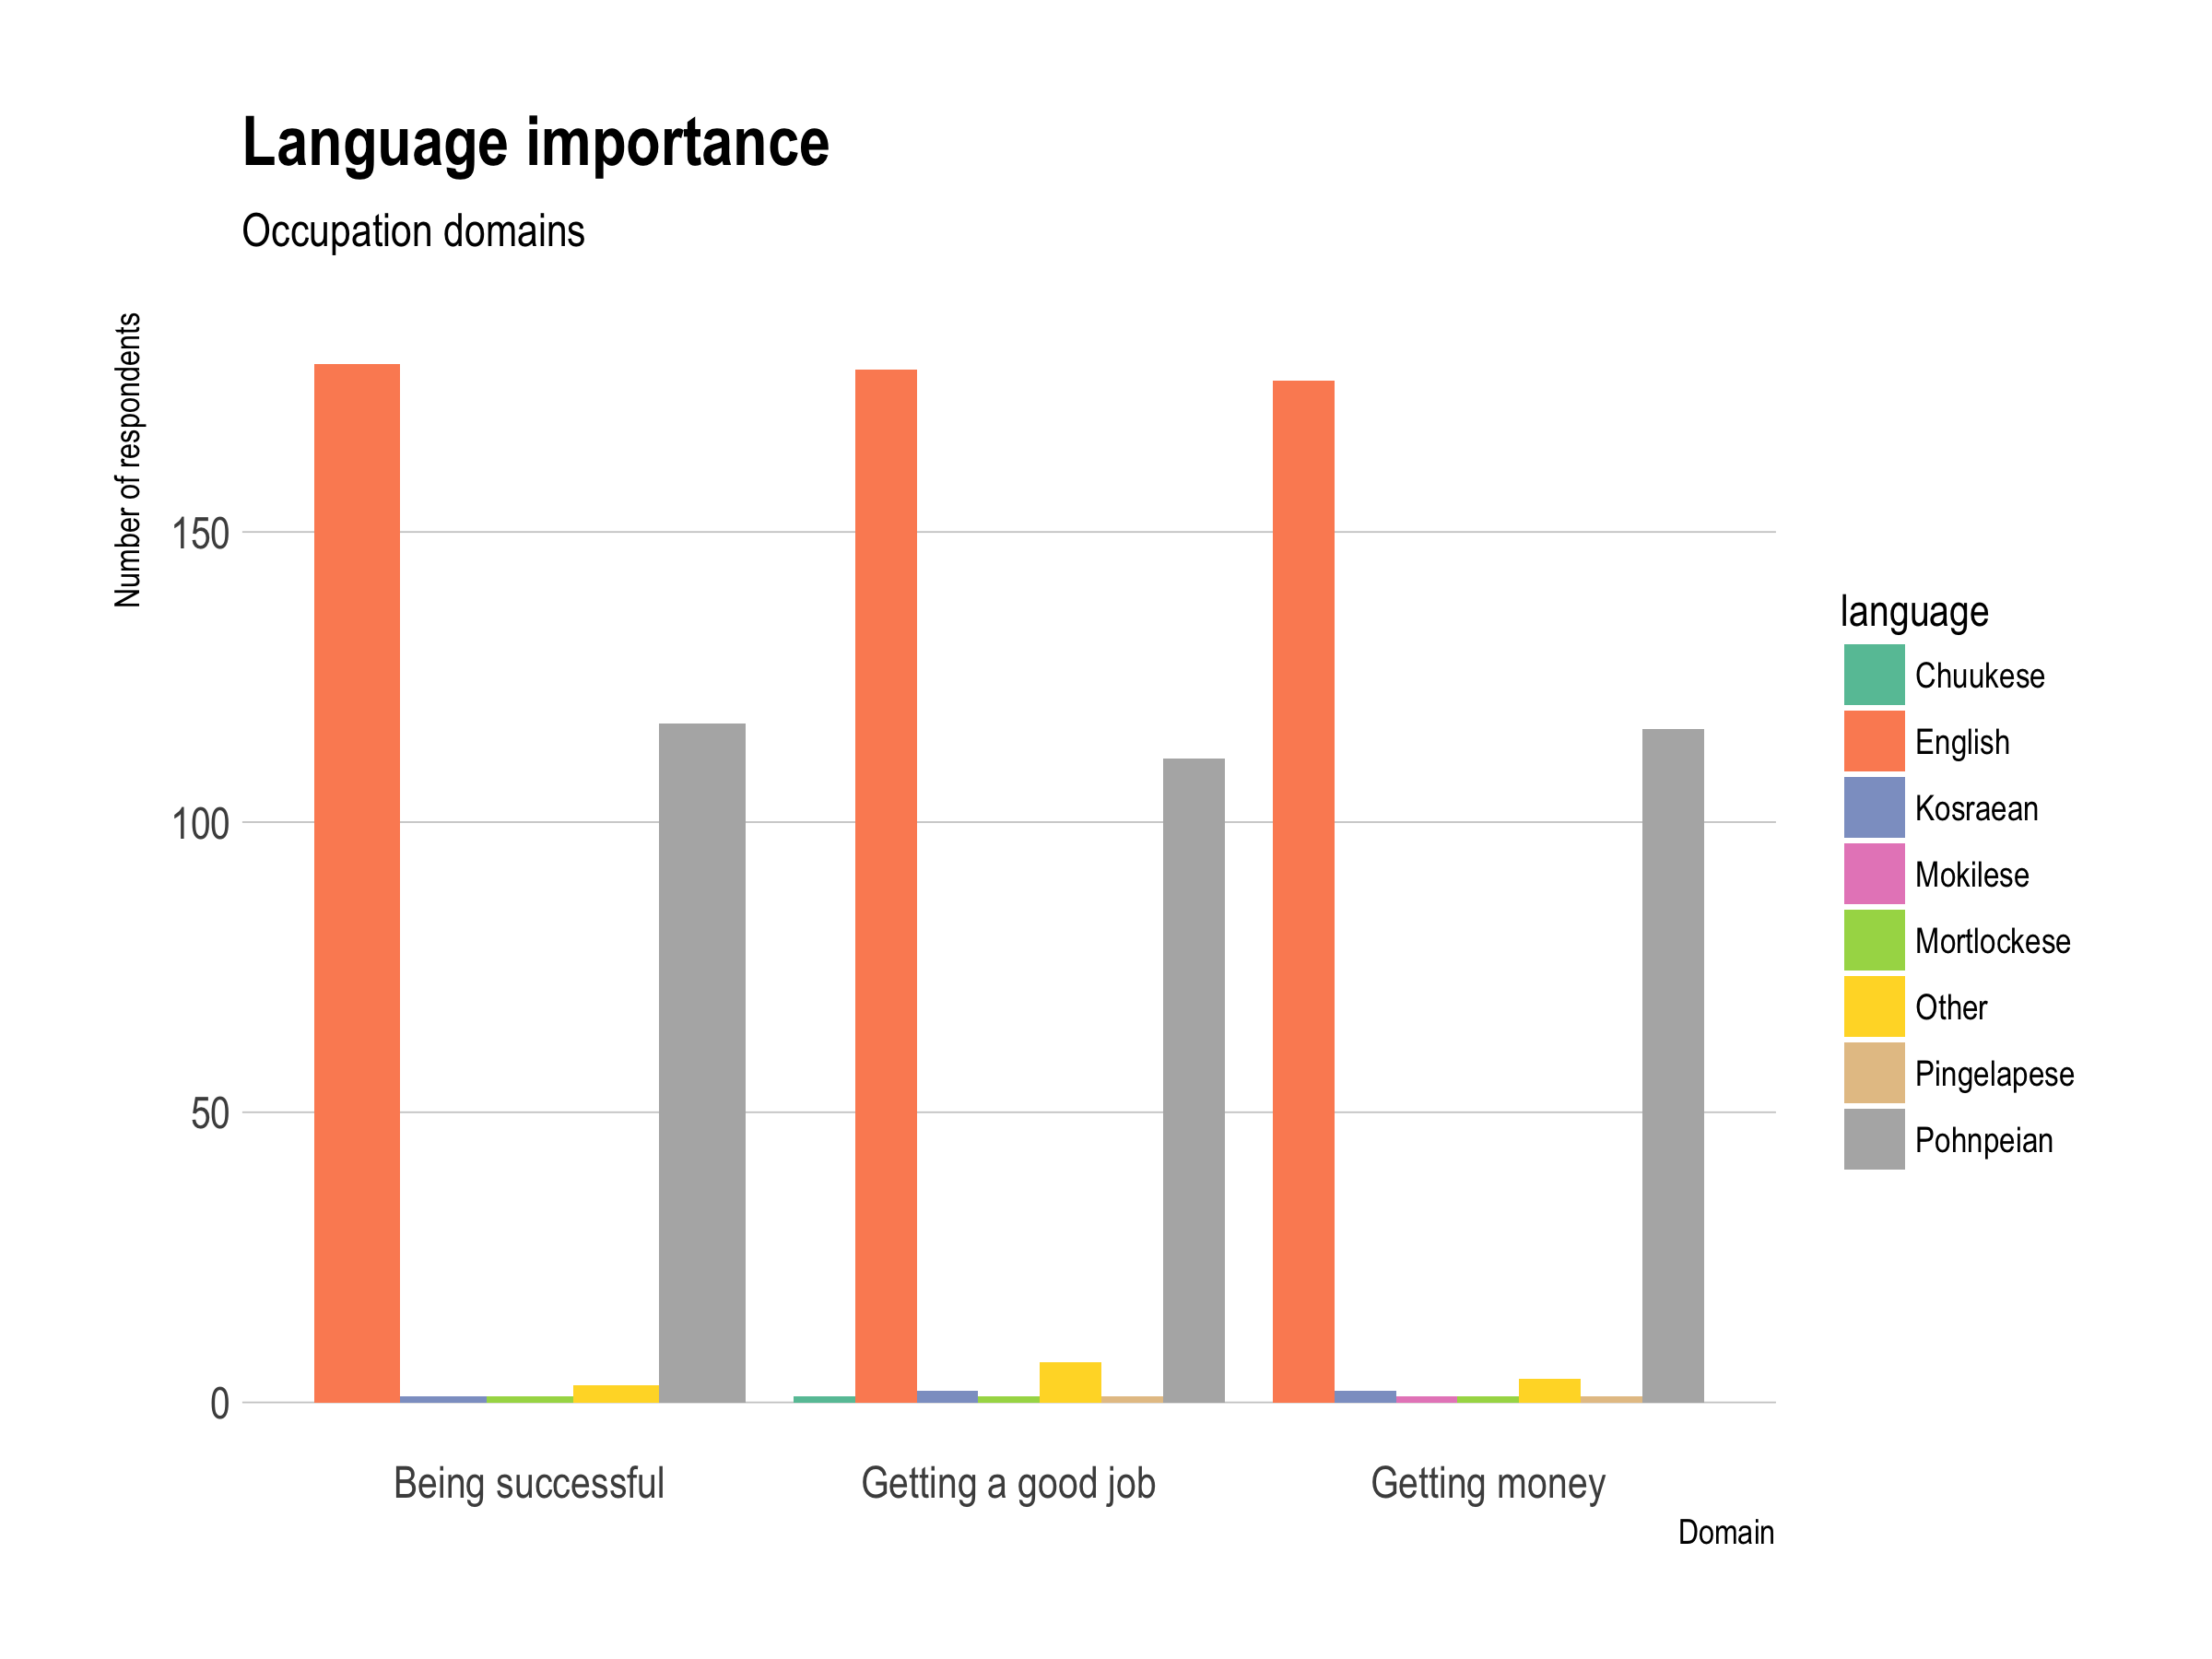
\includegraphics[width=0.9\textwidth]{figures/occupationdomains.png}
\end{frame}

\begin{frame}{PAM Occupation domains}
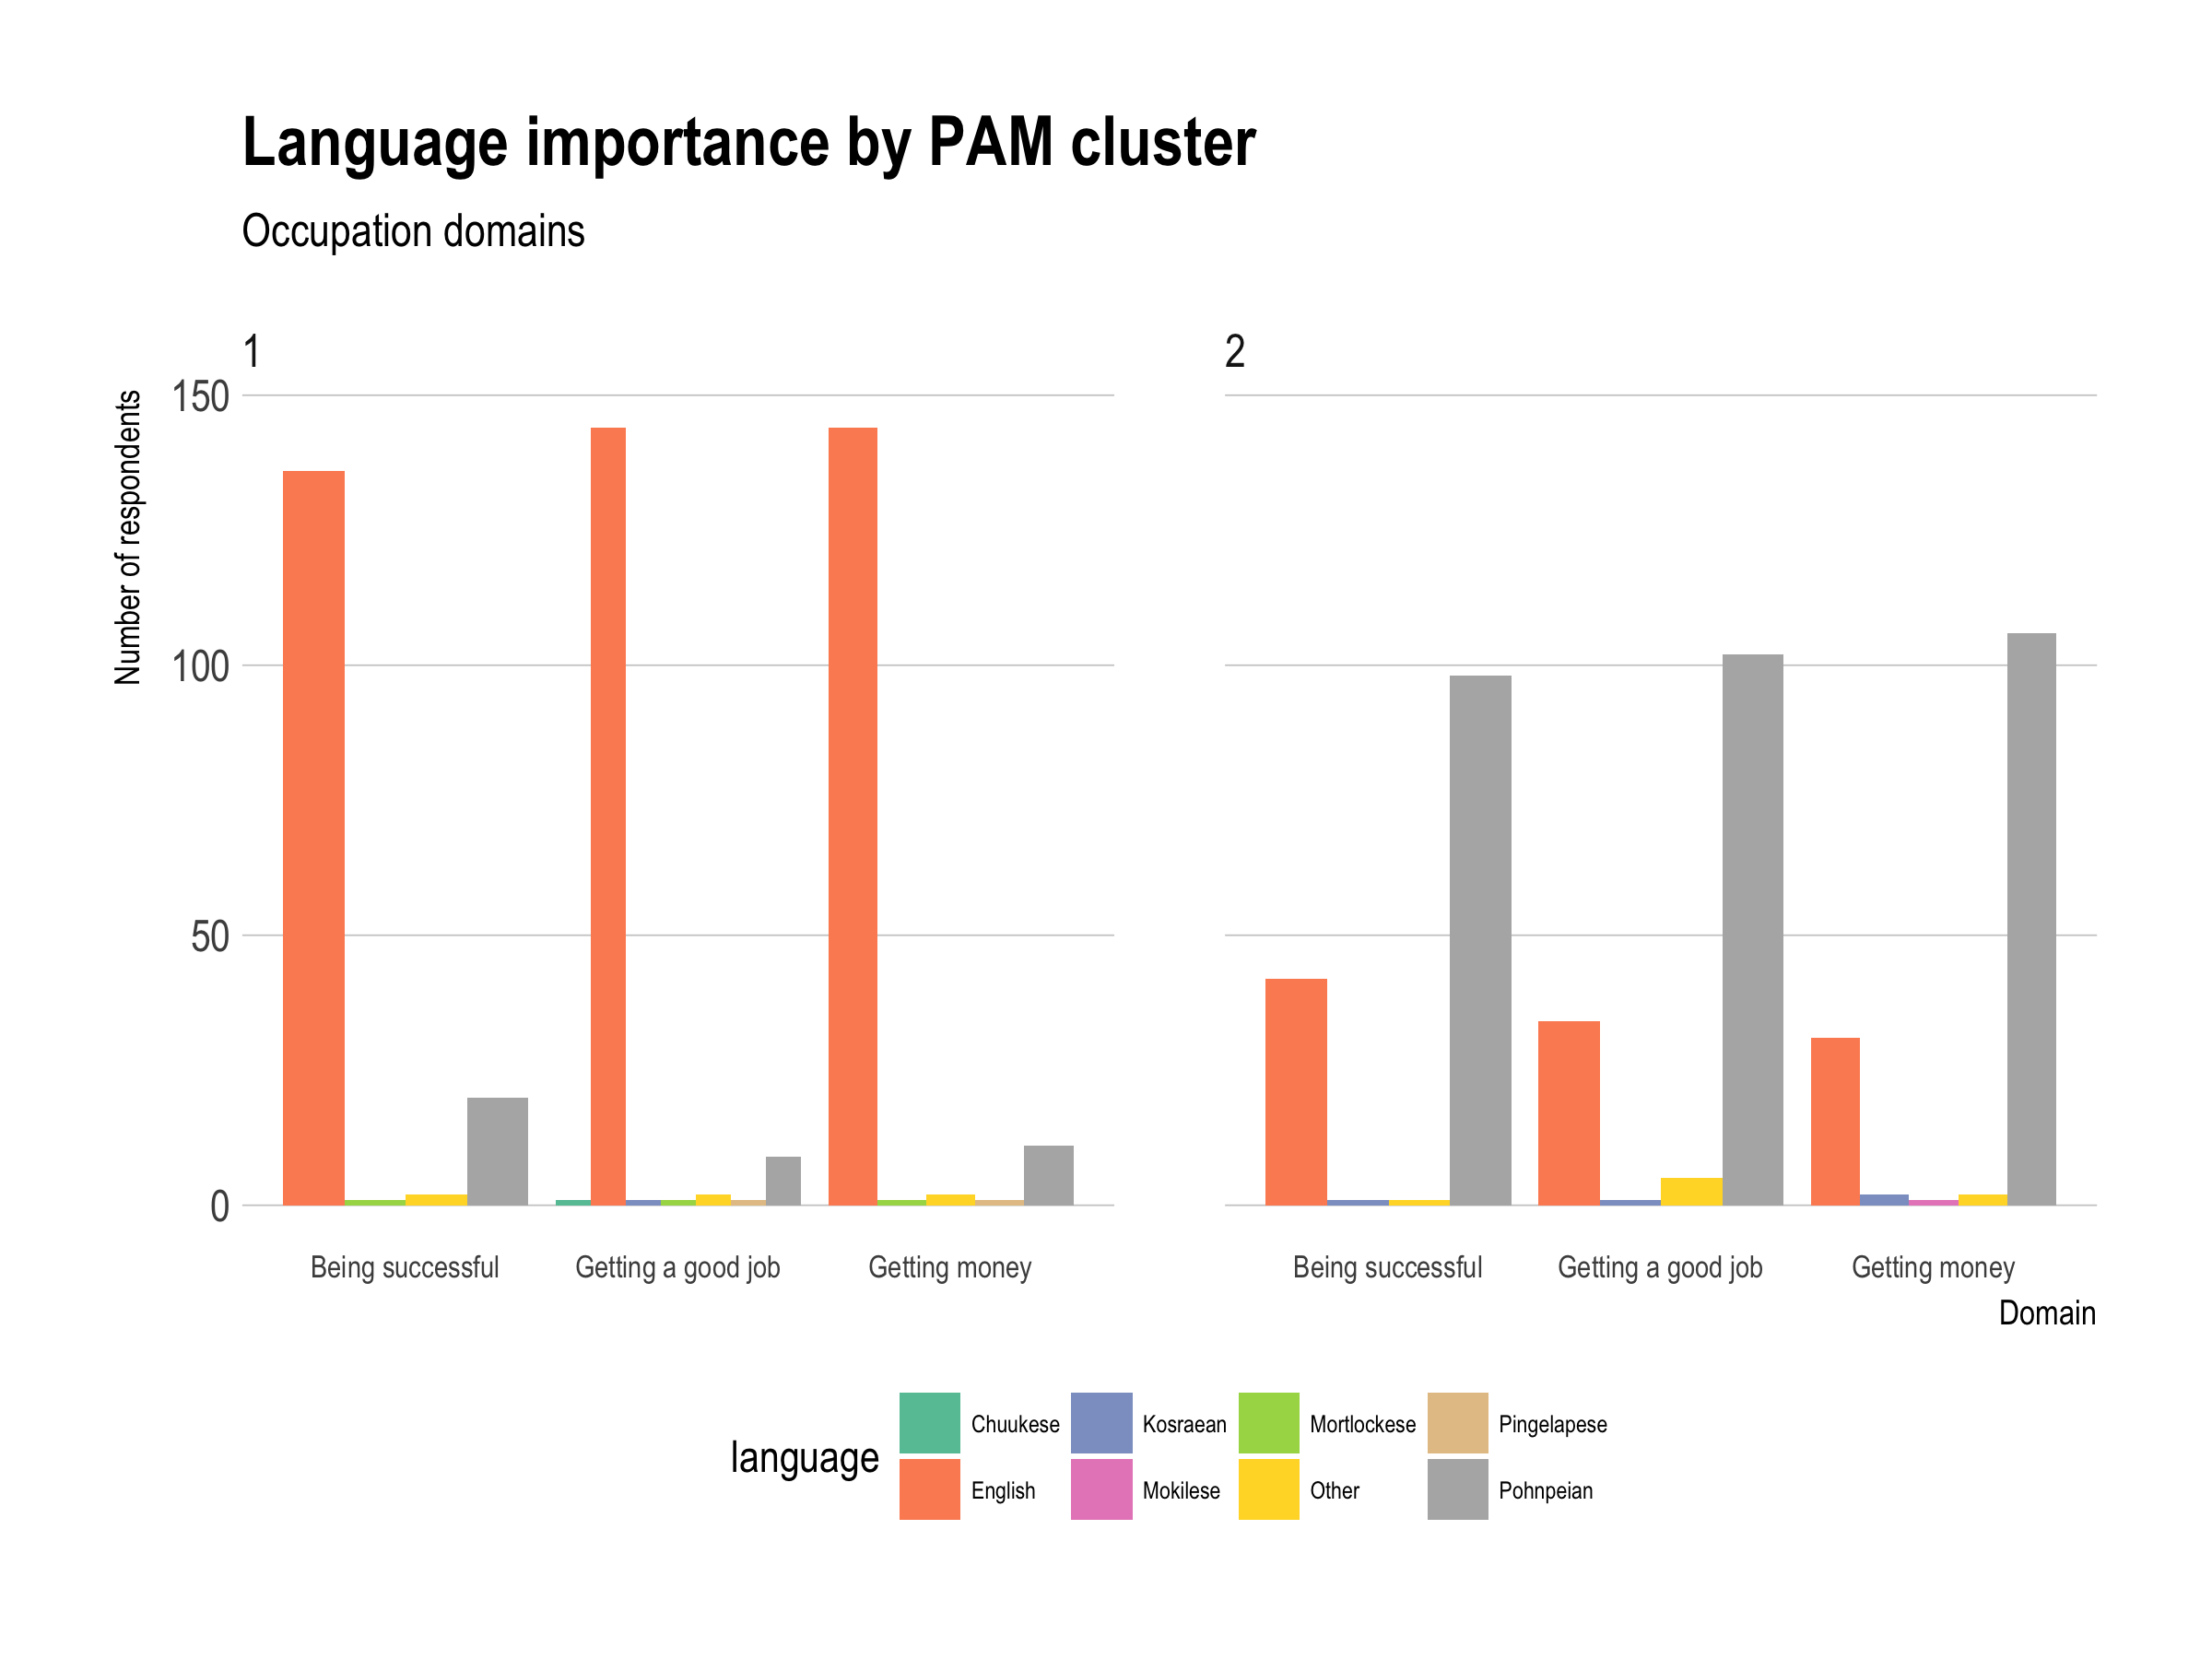
\includegraphics[width=0.9\textwidth]{figures/PAMoccupationdomains.png}
\end{frame}

\begin{frame}{General domains (original)}
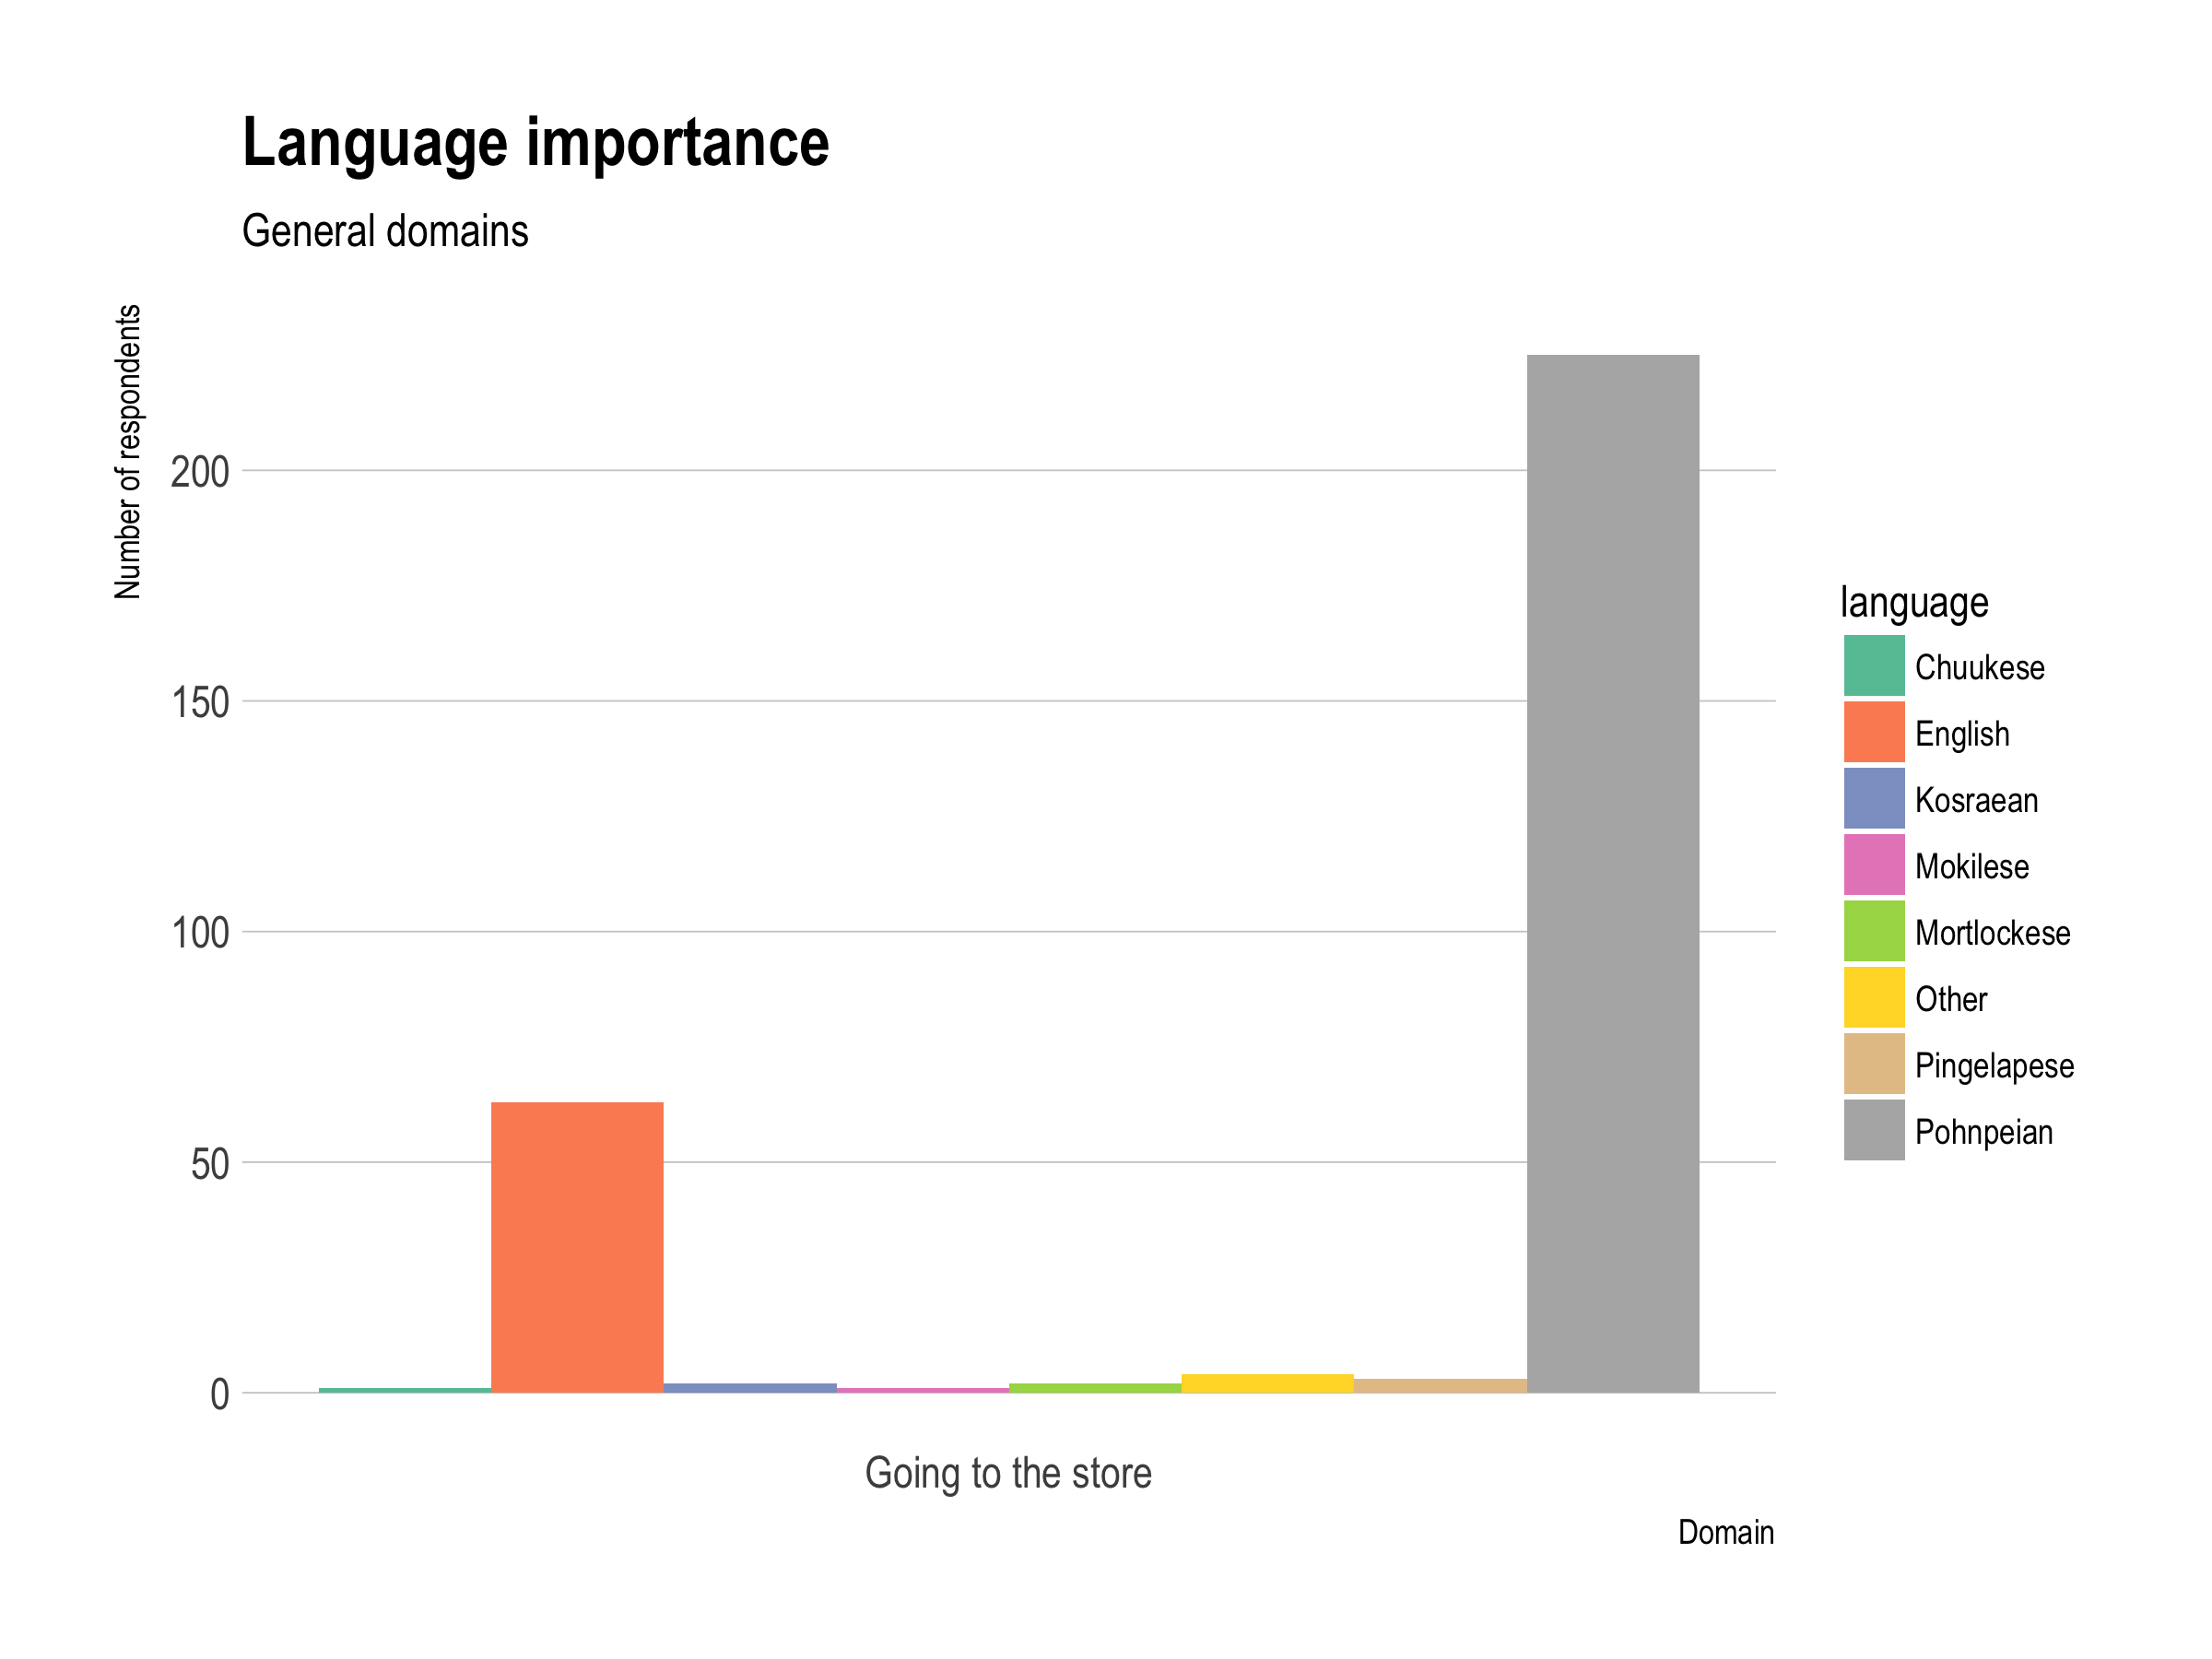
\includegraphics[width=0.9\textwidth]{figures/generaldomains.png}
\end{frame}

\begin{frame}{PAM General domains}
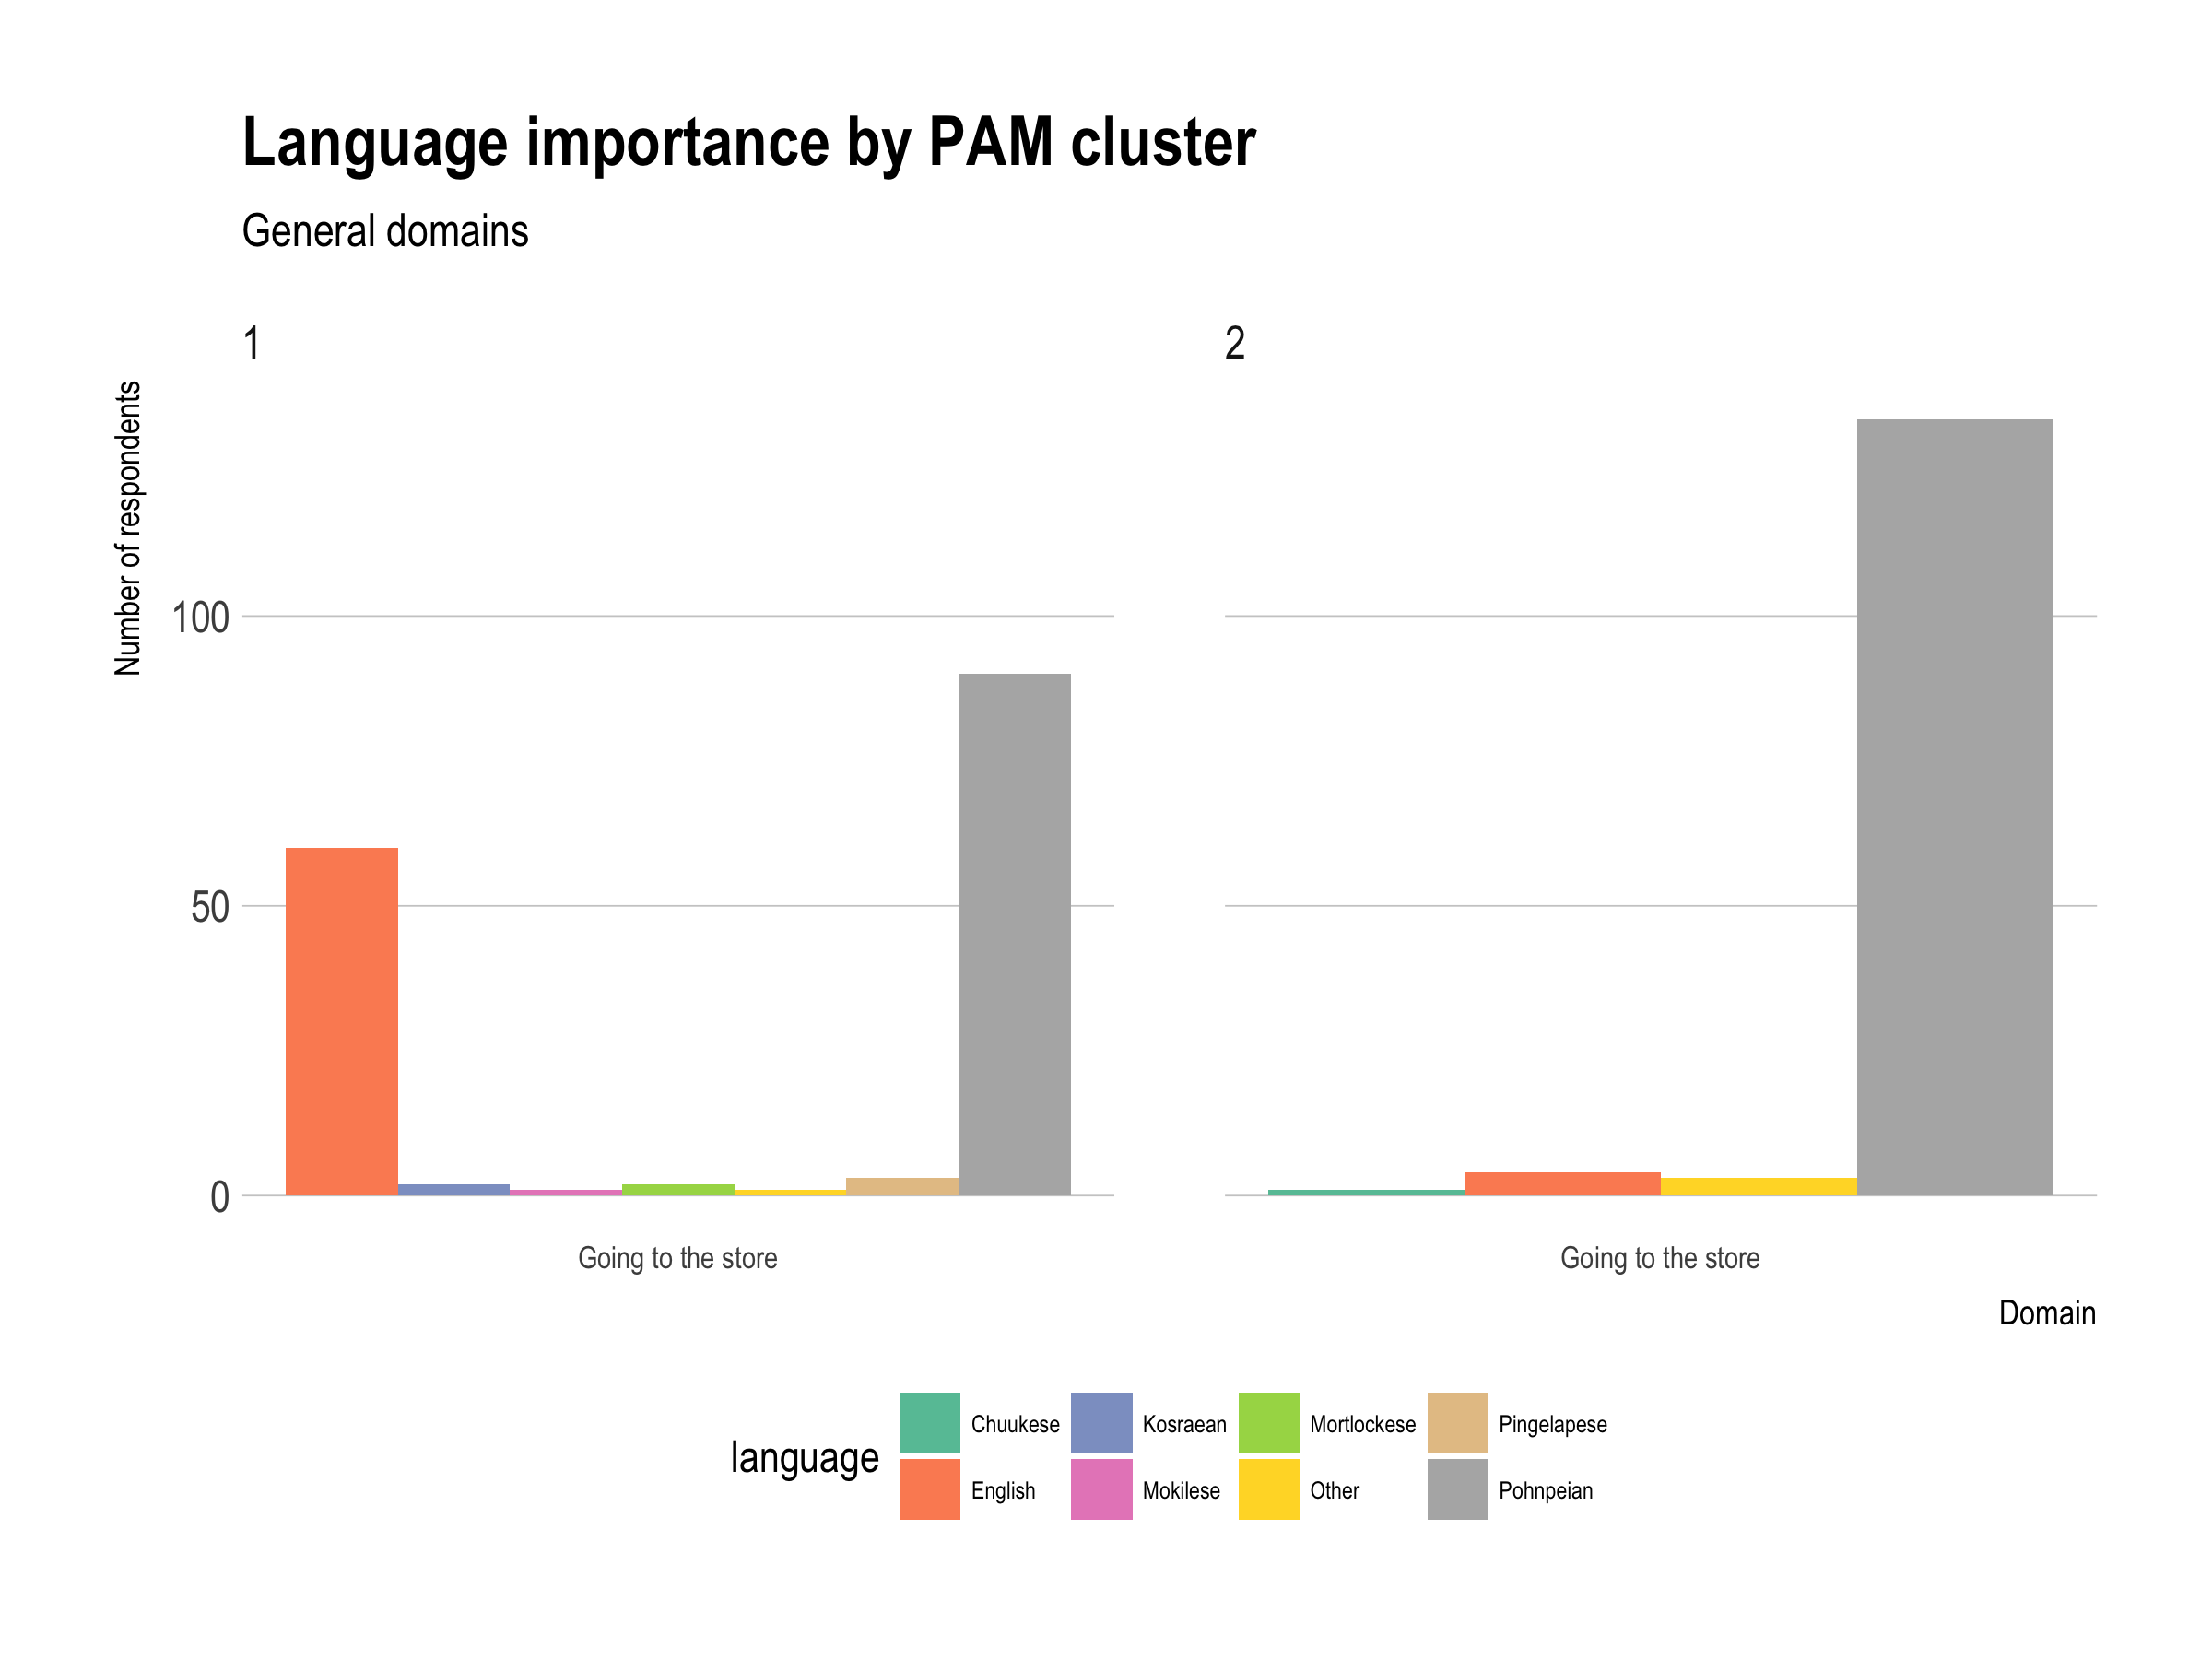
\includegraphics[width=0.9\textwidth]{figures/PAMgeneraldomains.png}
\end{frame}

\begin{frame}{Media domains (original)}
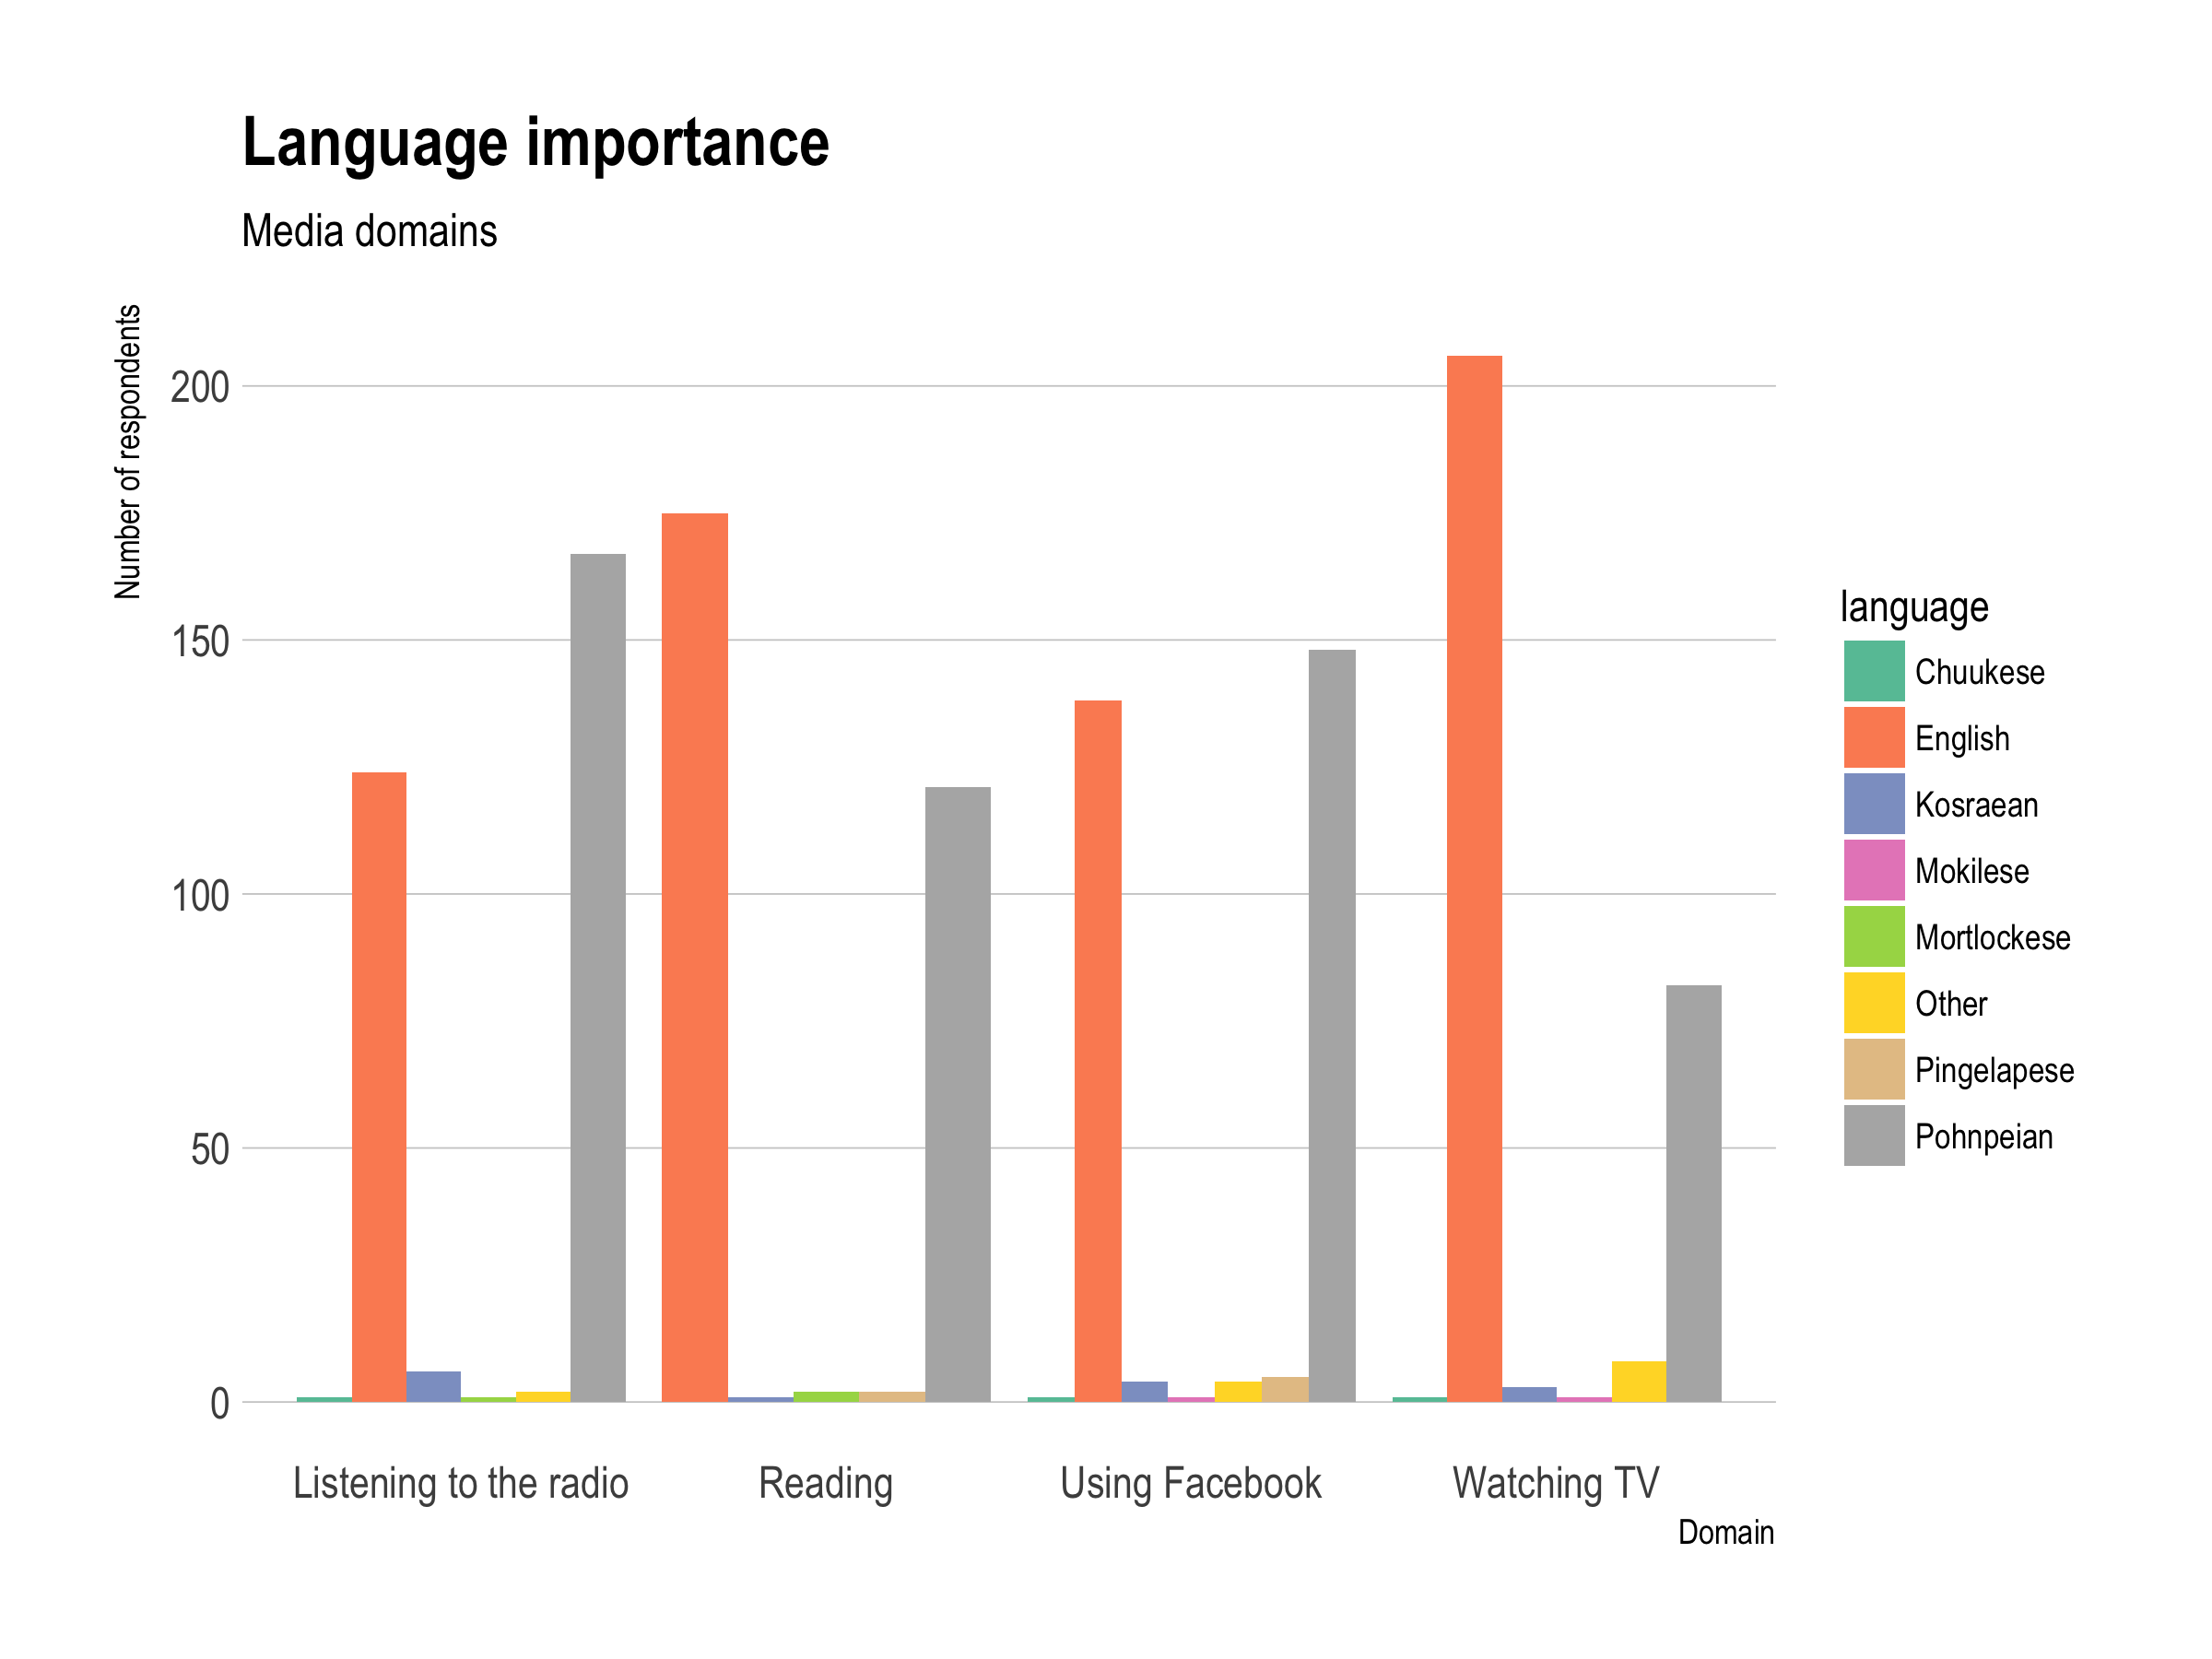
\includegraphics[width=0.9\textwidth]{figures/mediadomains.png}
\end{frame}

\begin{frame}{PAM Media domains}
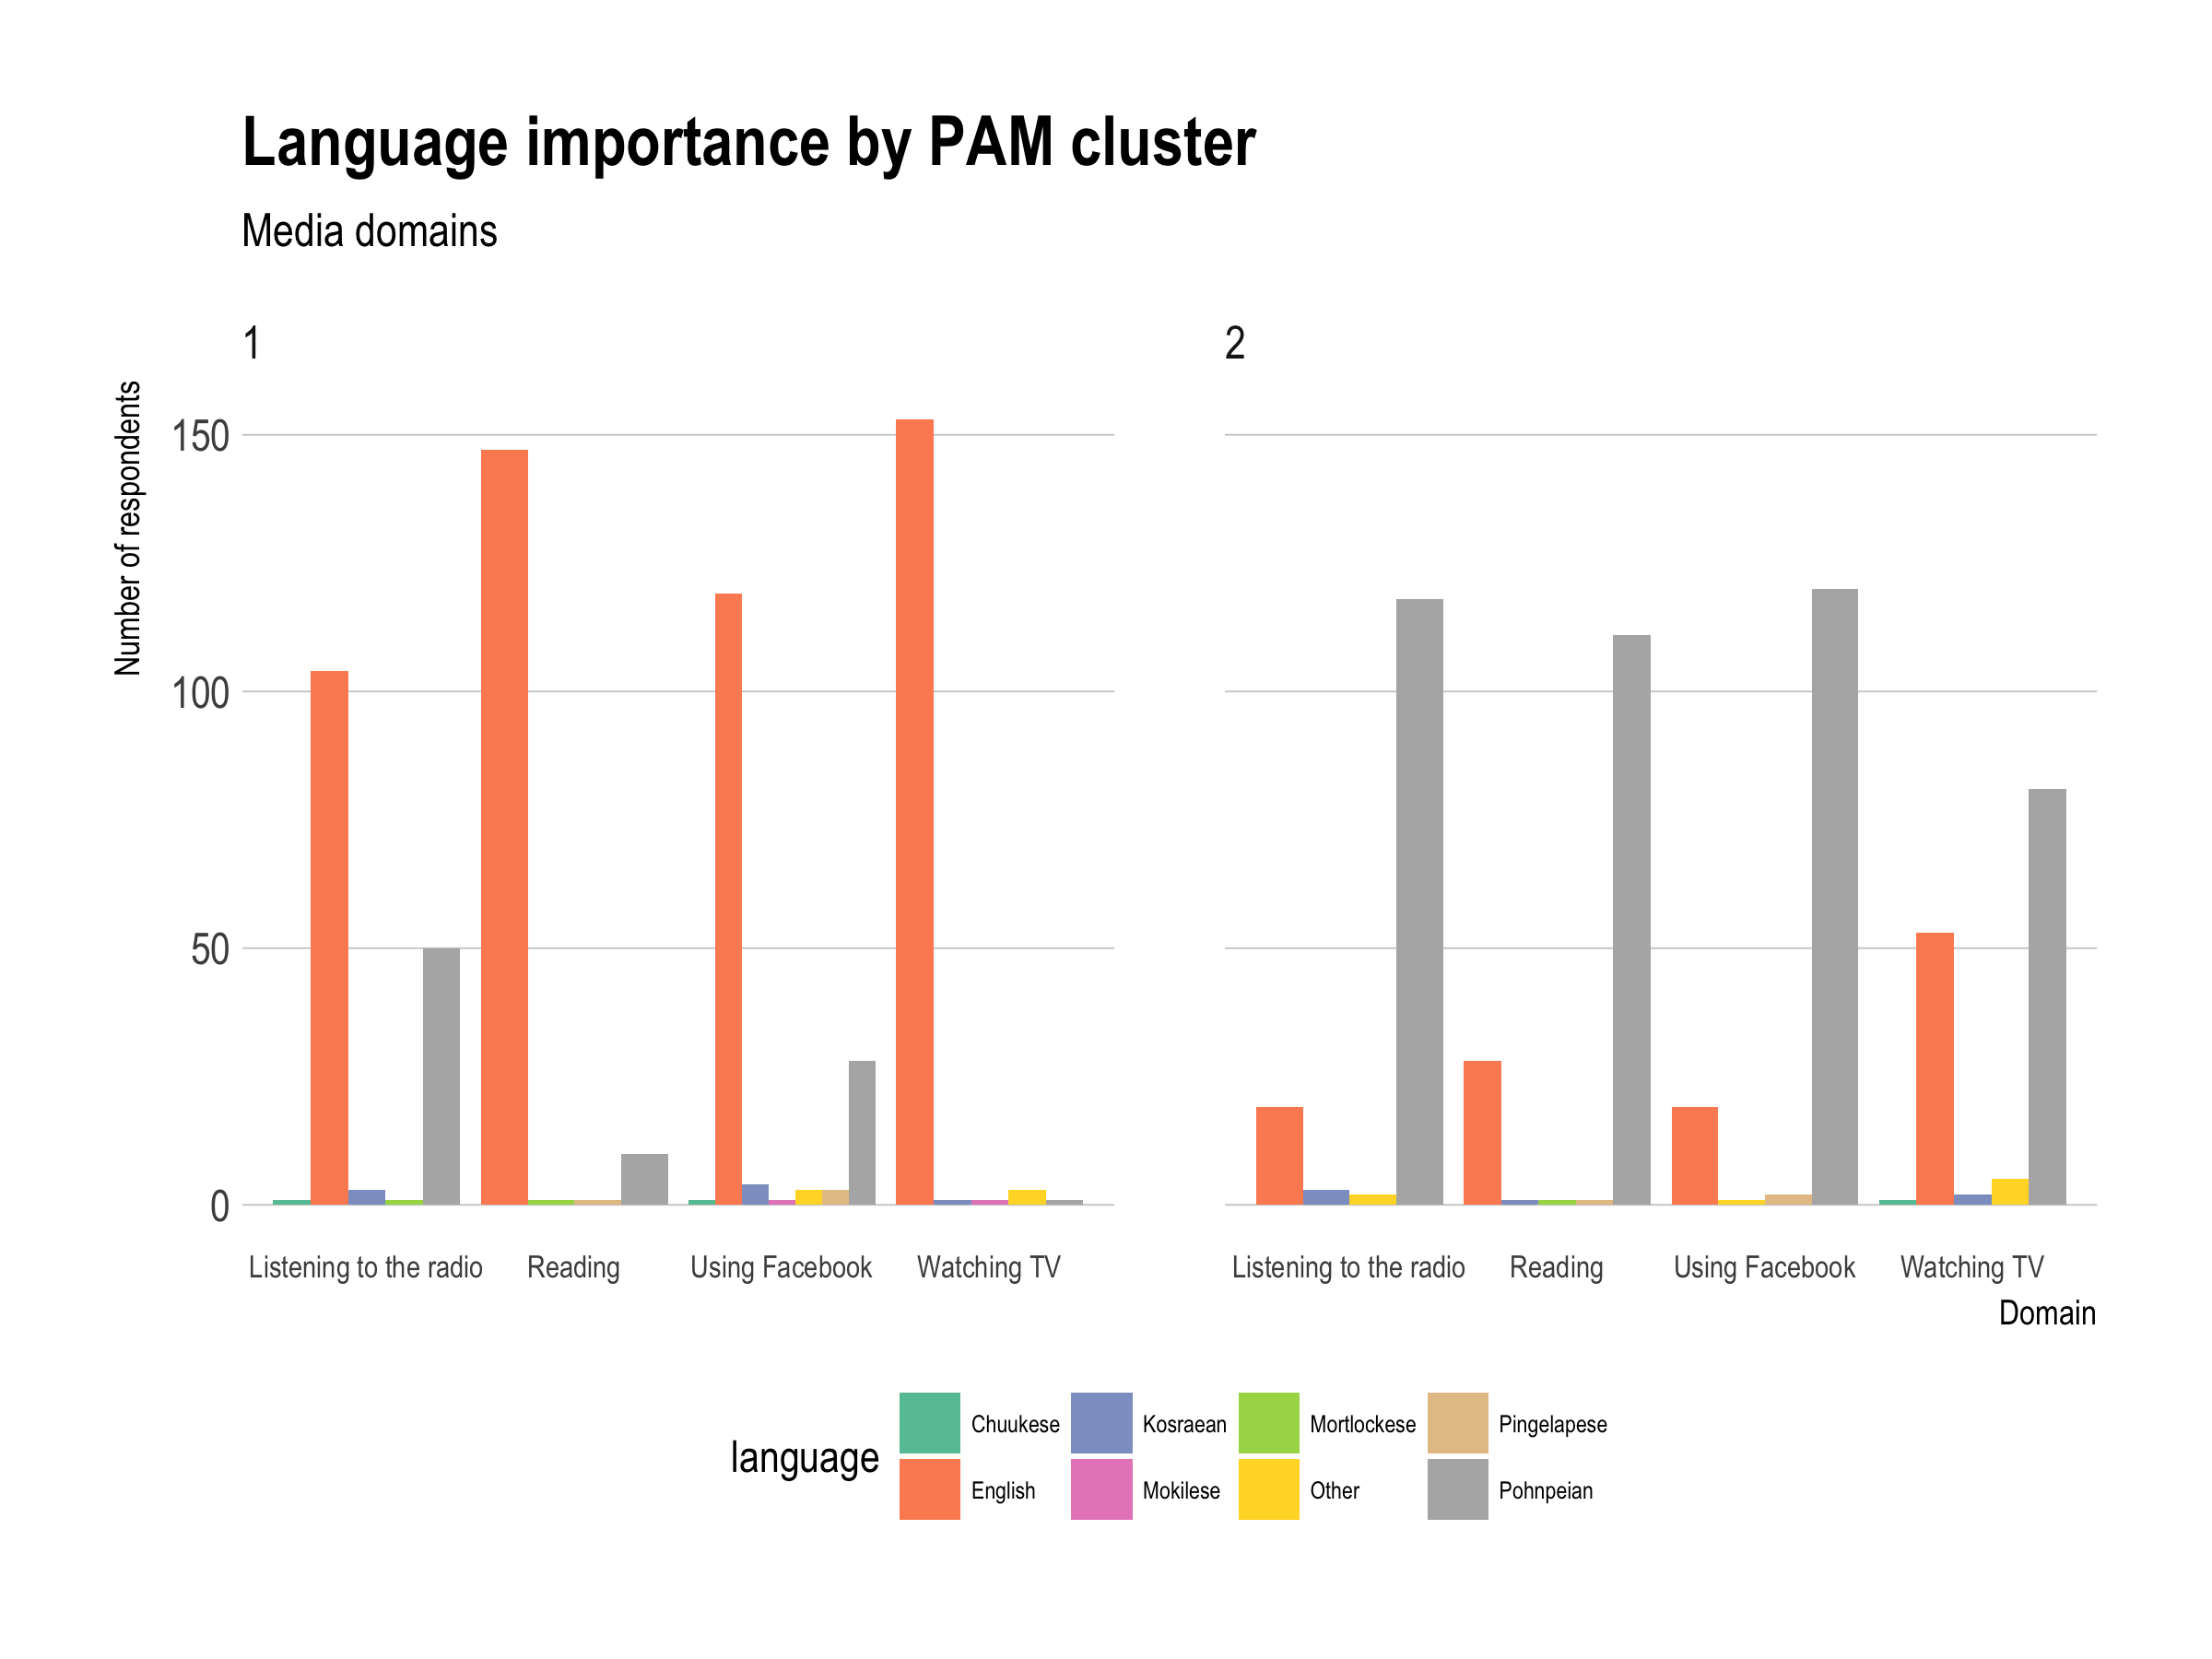
\includegraphics[width=0.9\textwidth]{figures/PAMmediadomains.png}
\end{frame}

\begin{frame}{Social solidarity domains (original)}
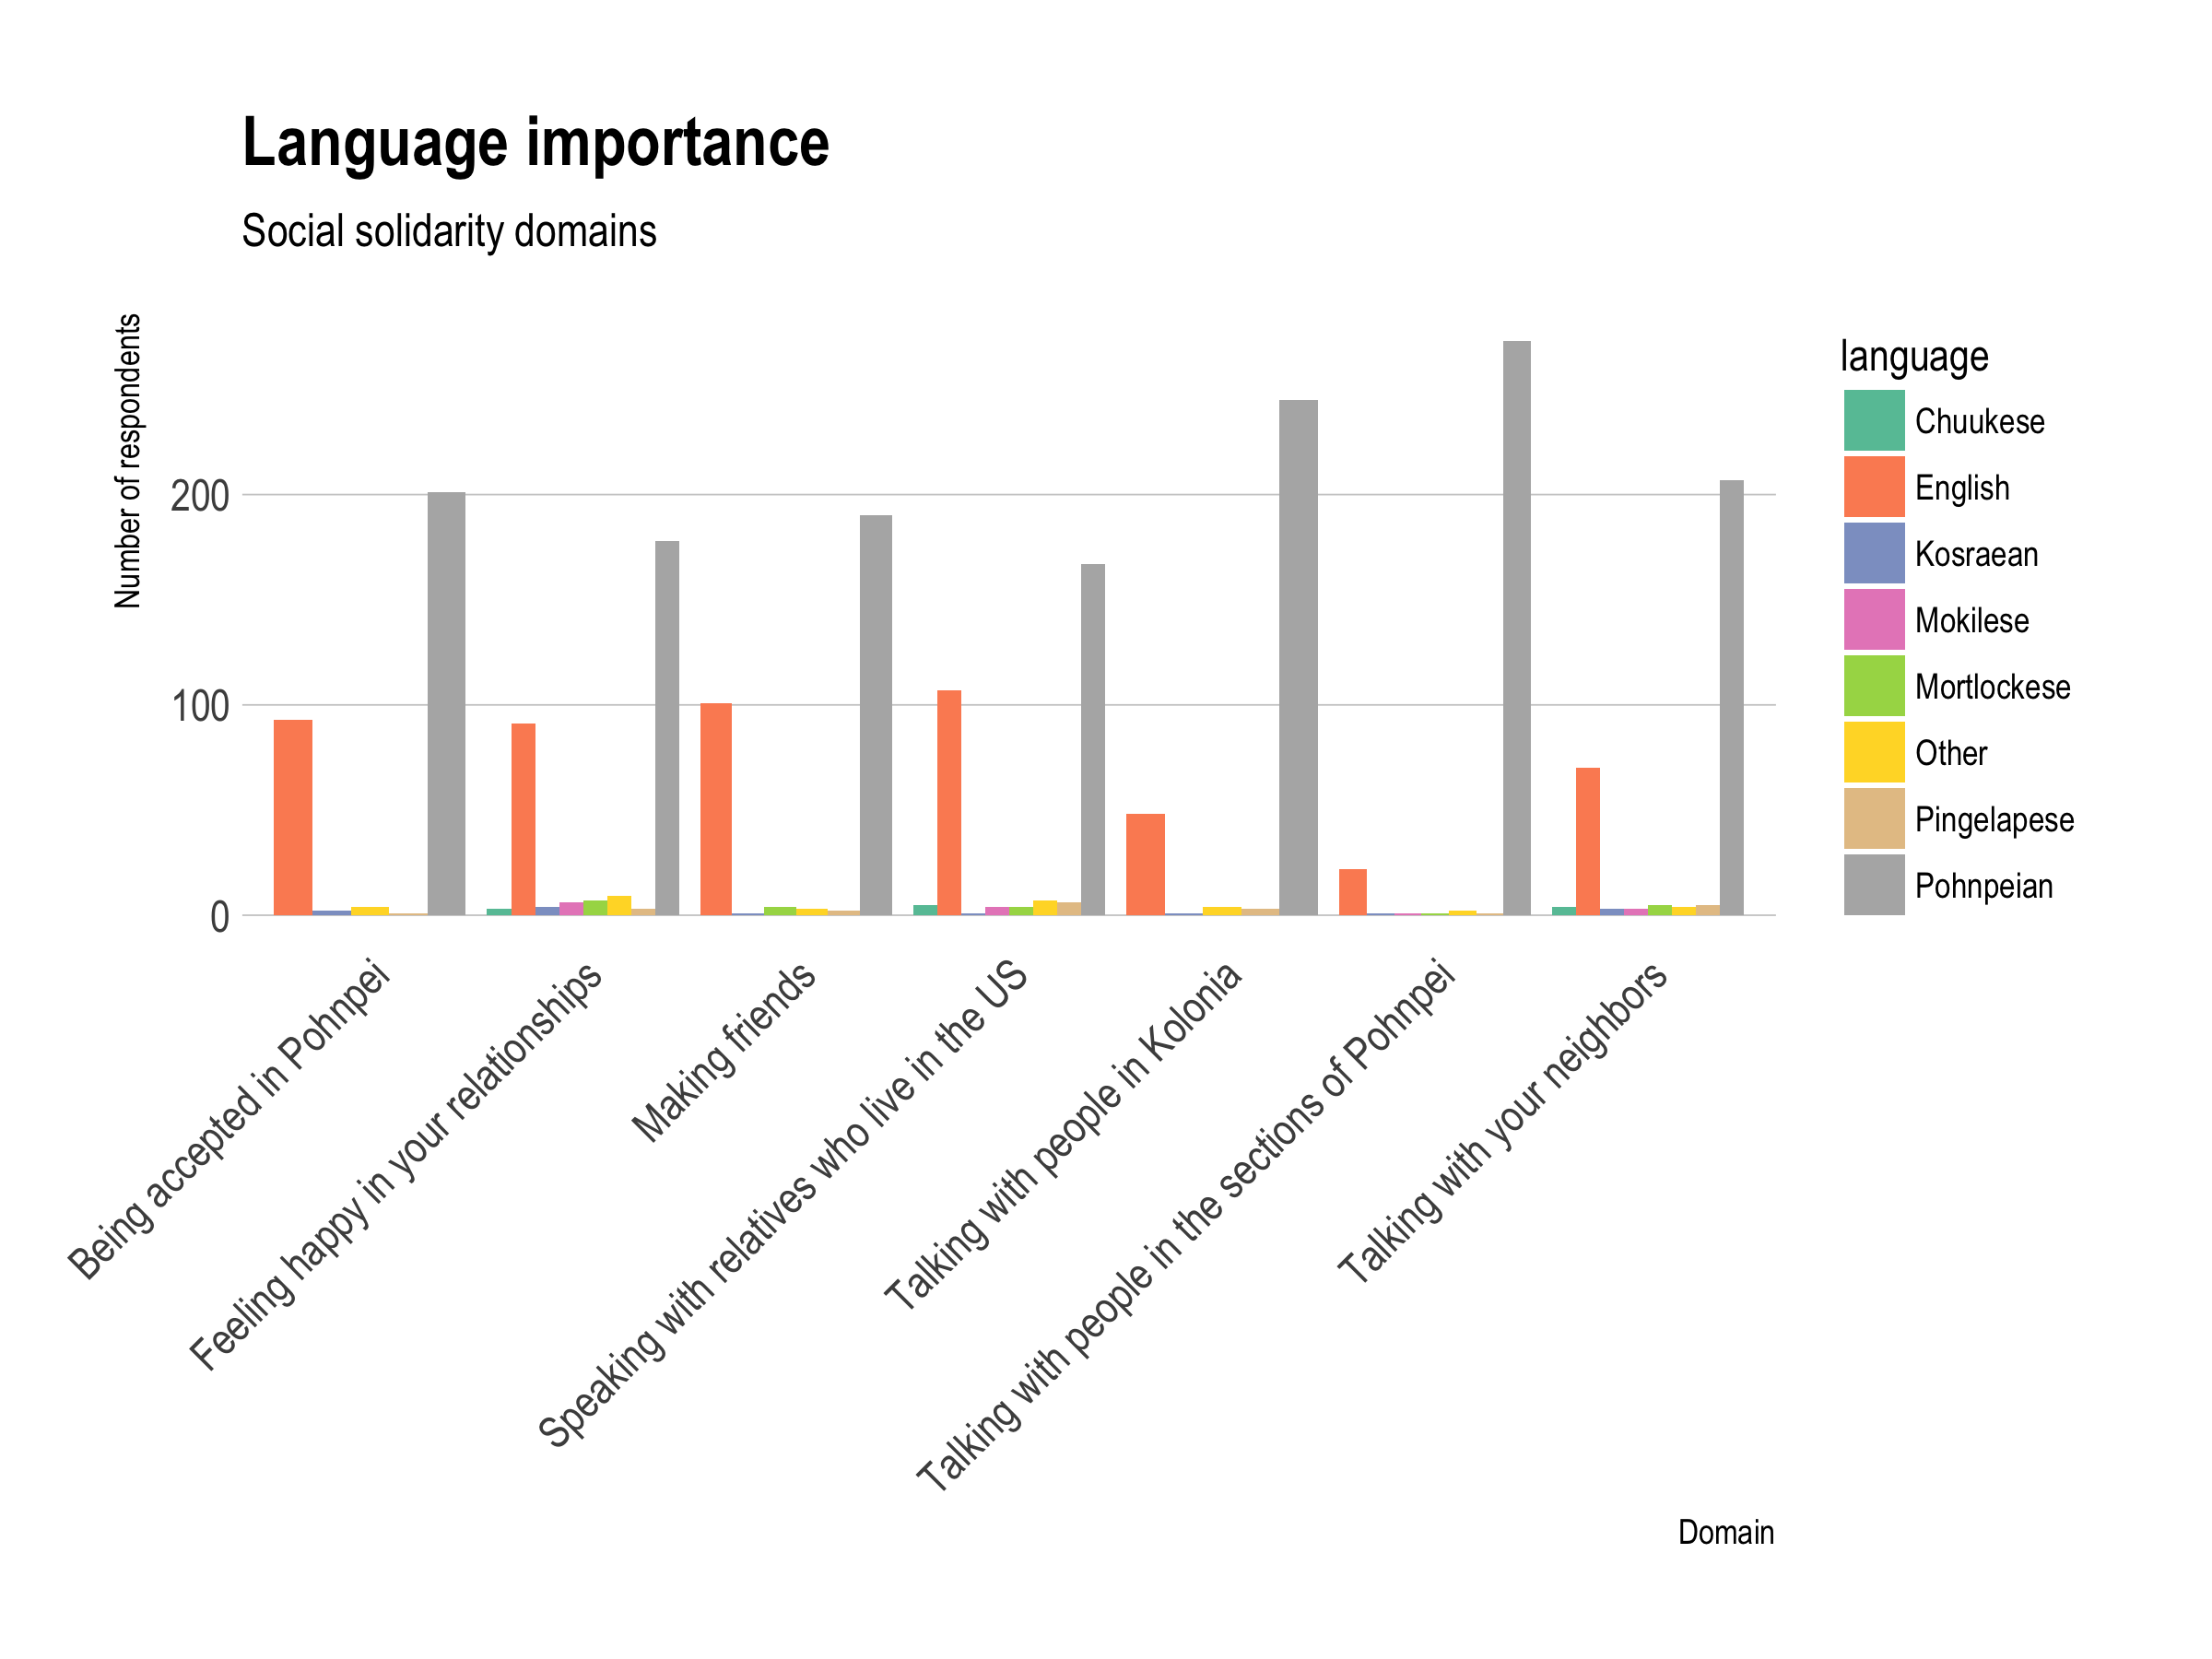
\includegraphics[width=0.9\textwidth]{figures/socialsolidaritydomains.png}
\end{frame}

\begin{frame}{PAM Social solidarity domains}
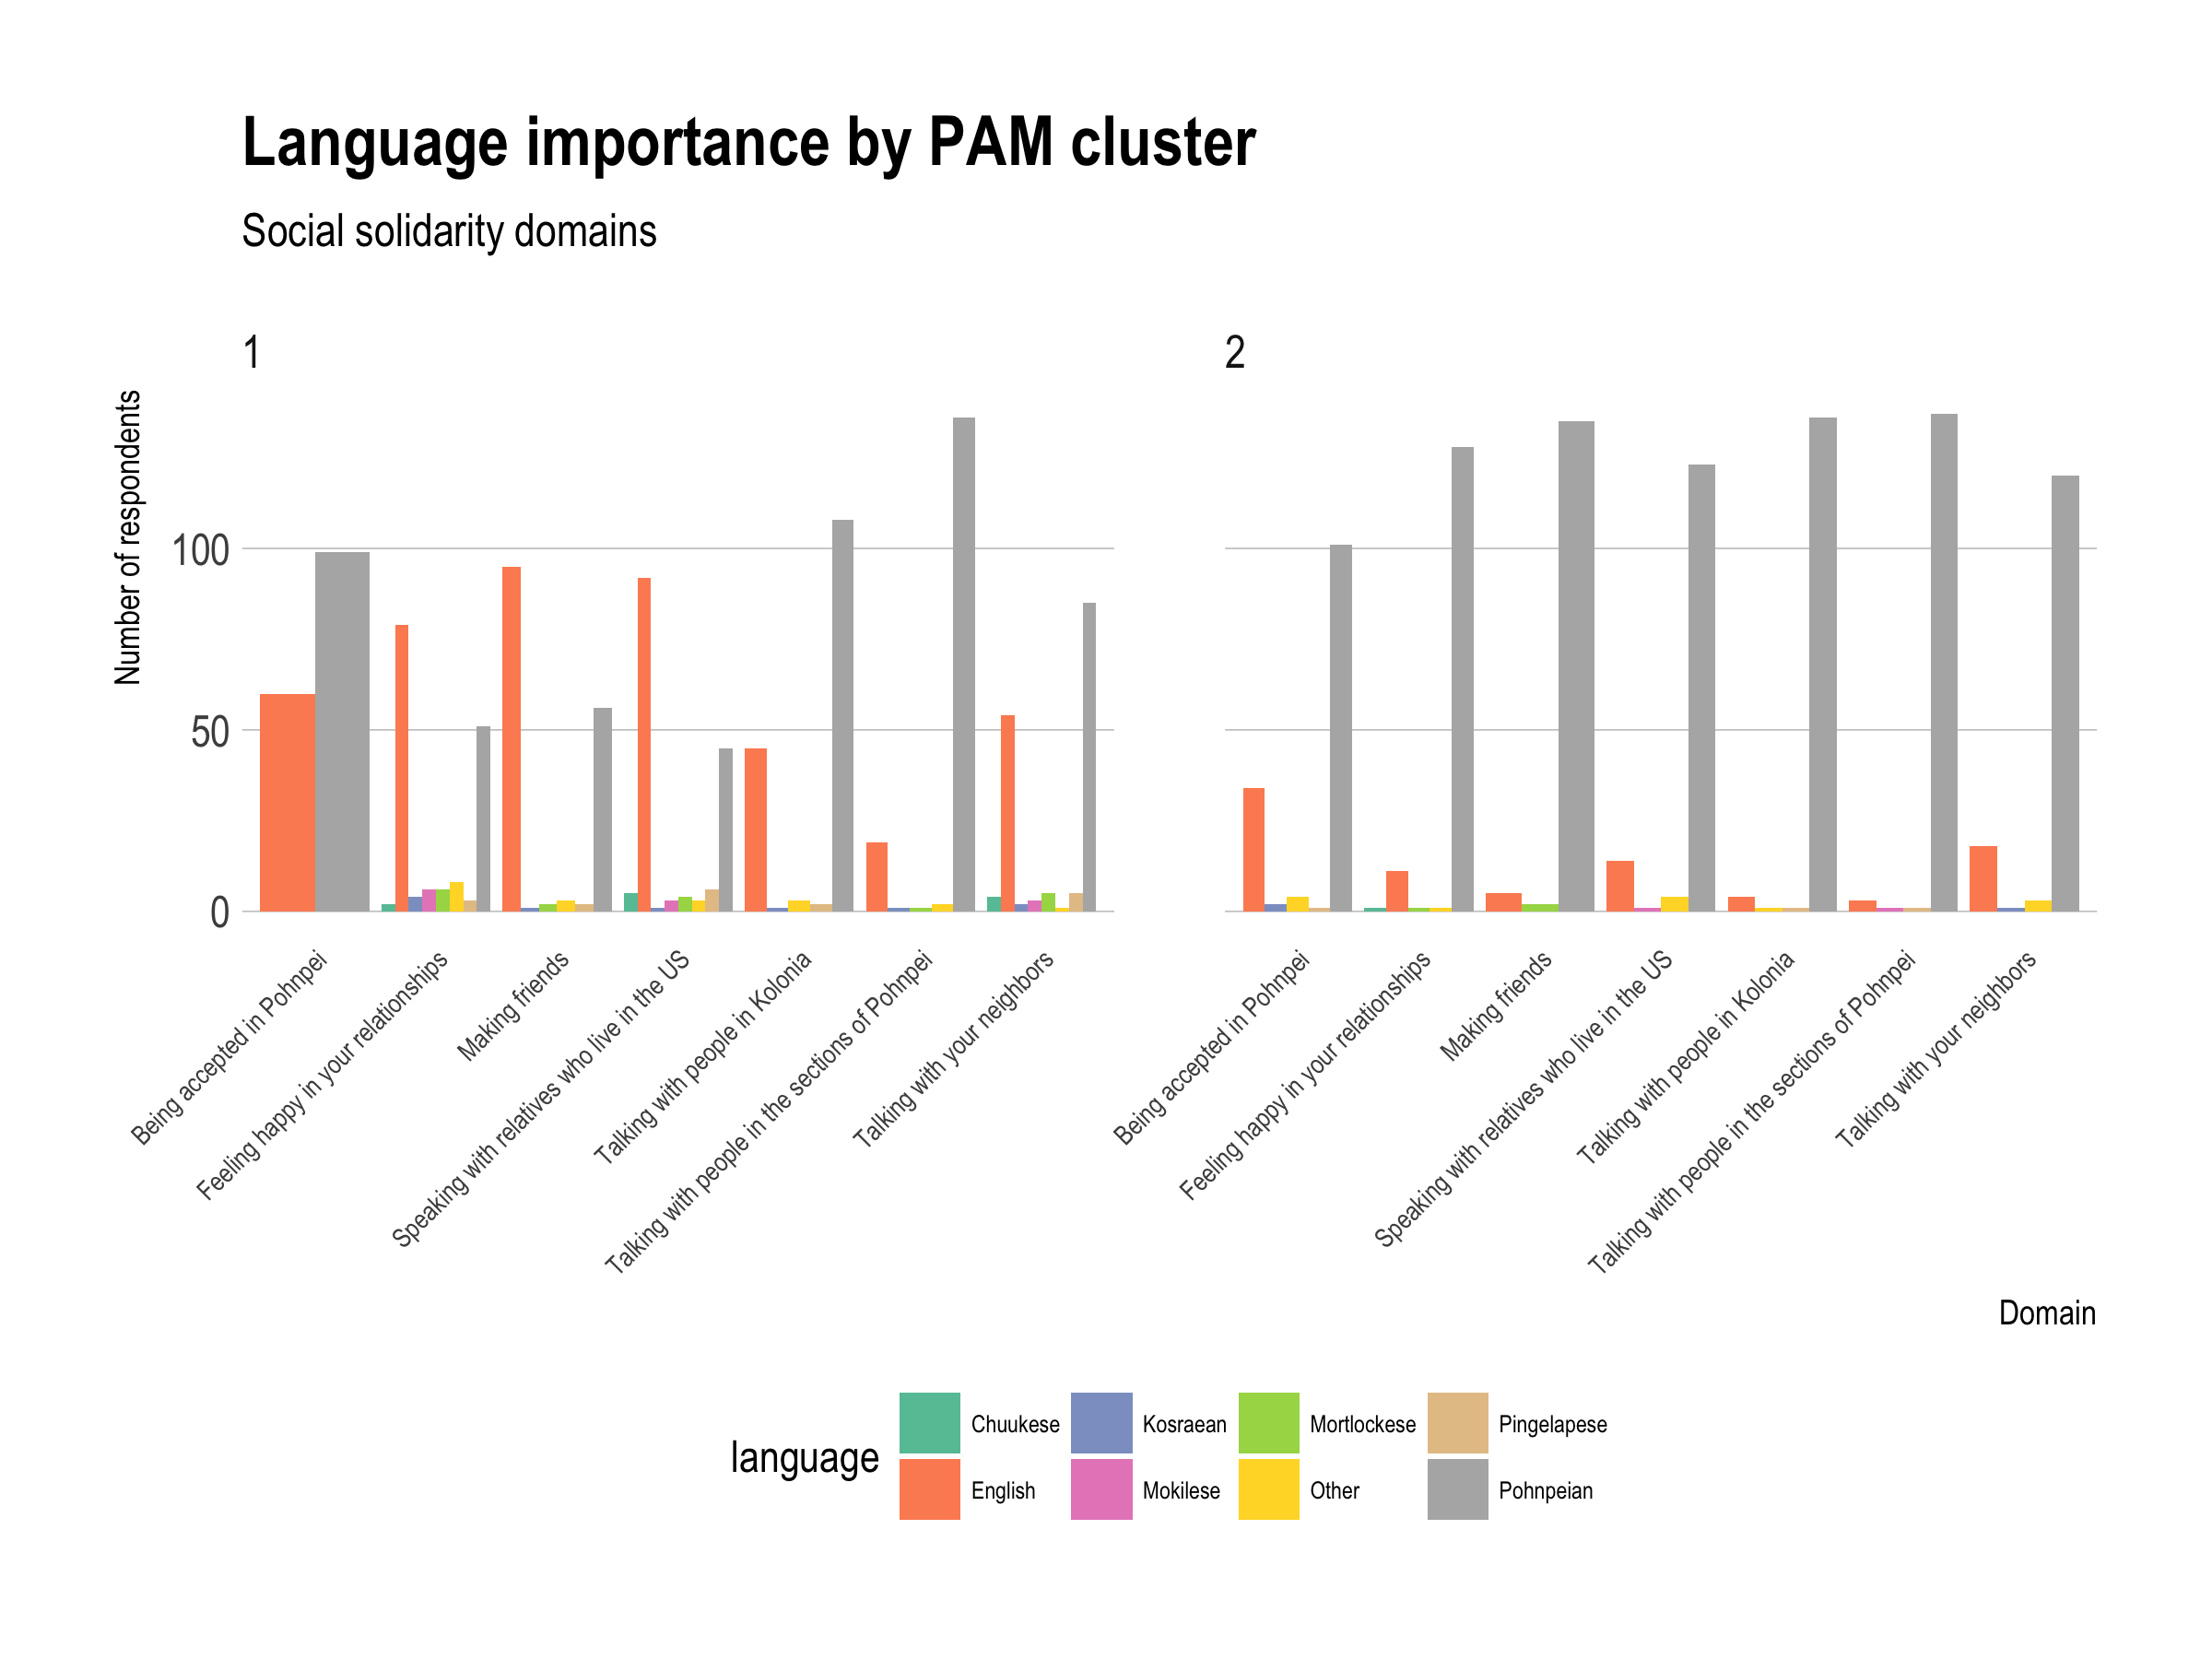
\includegraphics[width=0.9\textwidth]{figures/PAMsocialsolidaritydomains.png}
\end{frame}


\begin{frame}{Benefits of MDS and PAM}
\begin{itemize}
\item The data and analysis are not biased or limited by a priori groups
\item Shows groups and patterns that were hidden in the data and not shown by regression analysis
\item In this example shows two groups: one who values English over Pohnpeian and the other who values Pohnpeian over English
\item Also shows that even the English valuing group preferred Pohnpeian for some social solidarity domains (not limited to a single trend)
\item The resulting clusters can be analyzed post hoc to see if they correspond to specifc 
\end{itemize}
\end{frame}

\begin{frame}{Conclusions}
\begin{itemize}
\item Language attitudes research (and linguistics research in general) is about finding the categories and ideas the people actually use
\item One must be aware of the assumptions and limitations of the methods used, especially quantitative methods 
\item Using MDS and clustering analyses is one way to quantitatively allow local groups and categories to emerge from the data
\item It also helps paint a picture of the heteroglossia inherent in every community
\end{itemize}
\end{frame}

\begin{frame}{Kalahngan!}
Questions?
\end{frame}





\begin{frame}
%\section*{References}\vspace{-0.25in}\addcontentsline{toc}{section}{References}
\bibliography{prospectus}{}
\end{frame}


\end{document}